\documentclass[nofilelist]{cslthse-msc}
% to show a list of used packages at the end of the document, delete the nofilelist option
%\documentclass{cslthse-msc} 
\usepackage[utf8]{inputenc}
\usepackage[english]{babel}
\usepackage{amsmath}
%\usepackage{amsfonts}
%%\usepackage{amssymb}
\usepackage{amsthm}
%\usepackage{makeidx}
\usepackage{graphicx}
\usepackage[titletoc, header, page]{appendix}
\usepackage{transparent}
\usepackage{natbib}
\usepackage{booktabs}


% used to display the used files at the end. Select nofilelist as a package option to disable this
\listfiles % initialize

%\geometry{showframe}
%better like this?
%\student{Flavius Gruian}{Flavius.Gruian@cs.lth.se}
\student{Malte Kauranen}{dat14mka@student.lu.se}

\thesisnumber{LU-CS-EX: 2020-XX} % Birger Swahn will provide this number to you, once the thesis is ready for publication
% default is Master. Uncomment the following for "kandidatarbete"/Bachelor's thesis
%\thesistype{Bachelor}{Kandidatarbete}

%\title{Formatting a Master's Thesis}
\title{Cross-lingual comment toxicity classification}

%\onelinetitle
%\twolinestitle
\threelinestitle
%\fourlinestitle

\subtitle{Toxicity classification in newspaper comments and tweets}
\company{Ifrågasätt Media Sverige AB}
\supervisors{Gustav Hjärn, \href{mailto:gustav@ifragasatt.se}{\texttt{gustav@ifragasatt.se}}}{Pierre Nugues, \href{mailto:pierre.nugues@cs.lth.se}{\texttt{pierre.nugues@cs.lth.se}}}
%\supervisor{John Deer, \href{mailto:jdeer@company.com}{\texttt{jdeer@company.com}}}
\examiner{Jacek Malec, \href{mailto:jacek.malec@cs.lth.se}{\texttt{jacek.malec@cs.lth.se}}}

\date{\today}
%\date{January 16, 2015}

\acknowledgements{
I want to thank my supervisor Pierre Nugues for all the help and ideas I received during the making of the thesis. Making this thesis would also not be possible without the resources from Ifrågasätt Media Sverige AB in the form of a dataset, access to AWS and help with many other smaller issues from Gustav Hjärn, Henrik Fogelberg and several other people working at Ifrågasätt.
}

\theabstract{
The goal of this thesis is to explore the possibility for cross-lingual  classification of comment toxicity  with a focus on newspaper comments. For this purpose, I used a dataset from Ifrågasätt Media Sverige AB in Swedish to investigate if the newspaper comments are different in nature to other types of texts online. For the evaluation of the cross-lingual task, I used the OffensEval 2020 dataset. The results I obtained with the OffensEval 2020 dataset show that zero-shot toxicity classification, i.e. using a model trained on English text to classify Danish texts, is possible. However, it  performs poorly. We can achieve much better results by adding a small amount data in the target language (i.e Danish) to the training set. The performance is then similar to having a dataset of a similar size in only the target language i.e. training a model with only Danish text. In contrast, the differences in annotation standards and language in the Ifrågasätt Media Sverige AB dataset and the OffensEval 2020 dataset made their combination useless in cross-lingual training. This problem is potentially made larger due to the moderation guidelines creating a gray zone or missing context in the Ifrågasätt Media Sverige AB dataset.
}

\keywords{Natural language processing, Machine learning, Toxicity, Offensive text classification}

%% Only used to display font sizes
\makeatletter
\newcommand\thefontsize[1]{{#1 \f@size pt\par}}
\makeatother
%%%%%%%%%%

\begin{document}
\renewcommand{\bibname}{References}

\makefrontmatter
\chapter[Introduction]{Introduction}
\section{Background}
As the usage of the internet continues to grow, so does the discussion between individuals on it. People in a wide variety of forums talk to each other and interact with more ease and in different ways than before. In some ways this is positive: More people interacting and discussing things can lead to constructive dialogue. Some social media are almost entirely centered around comments with them filling an essential role for sites such as Facebook or even being almost the entire platform as in the case of Twitter. 

However, these conversations often turn into vile attacks and nonconstructive discussion. To prevent their platform from being swamped with poor comments, many websites decided to moderate these discussions. Due to the enormous amounts of data, it is not practically possible for people to manually check if all the content on these platforms is acceptable. It has therefore garnered public interest on whether we can apply text classification techniques. There have been many recent public evaluations who have tried to tackle this problem. The OffensEval 2019 competition is an example of them that was based on Twitter data \citep{zampieri2019semeval}. This public competition and others have shown that these techniques are not perfect and cannot guarantee reliably that they will remove toxic content.

More traditional media have also tried to embrace comments on their platforms with the potential of increasing user engagement and adding value to the information being reported. However, emerging toxic comments on the platforms clash with the newspapers duty to prepare well-researched and informative texts. While the comments are not necessarily the editorial responsibility of the newspaper when published, a comment under an article  affects every reader's perception of this article. 

This means that comments on newspapers sites have different requirements to provide value to the customer. Newspapers comments  generally need to uphold a higher standard than on other types of social media. In practice, this higher standard of debate has failed to materialize. This led many newspapers to remove the comments because the content that emerged did not complement the reporting of the newspaper \citep{trygg2012comment}. Due to need of an around-the-clock large moderating team, moderating proved too expensive for its return on investment.


Ifrågasätt Media Sverige AB tries to solve these problems by providing a centralized platform for newspapers. A few employees work to provide moderation during all times of the day, making it easier for individual newspapers to start having comment fields without facing the large upfront costs of moderating a comment field. To do this, Ifrågasätt uses a partially automated process:
\begin{enumerate}
    \item The platform immediately publishes all the comments;
    \item  Moderators read and label all the comments, but prioritize those flagged by an automated system.
\end{enumerate}

The automated system assumes all comments are in Swedish. It is only capable of meaningfully giving a rating to those that are wholly in Swedish. Up until recently, this has not been a problem as all publications have been in Swedish. However, this prevents Ifrågasätt from effectively operating in countries other than Sweden. 

The objective of this Master's thesis is to explore the potential of moderating comments in other languages and if it is possible to expand the automated moderating system to them.


\chapter{Theory}
There are many different ways to address cross-lingual text classification. This chapter aims to delve into some of the approaches commonly used with machine learning, quickly explain the theoretical foundations for them, and motivate why they can be used for the Ifrågasätt dataset.

The problem of expanding the system to other languages can be divided into two parts:
\begin{enumerate}
    \item The first one is the text classification problem. Texts from another language have to be classified into either a non-toxic or toxic category. 
    \item The second part addresses the transfer learning from the Swedish dataset: Is it possible to learn and use features from the Swedish language dataset to train a model in another language? 
\end{enumerate}

The second part of transfer learning requires that some of the foundations of the text classification problem have been settled. I will then first outline the theory behind the text classification. As I will show, some existing models have already tried to answer this question. 

\section{Text Classification}

While there are many algorithms for text classification, they are all centered around two things:
\begin{enumerate}
    \item Learning features from the text, i.e. learning pieces of information that are relevant for determining what class the text is and then
    \item Combining those to make a decision on which class the text belongs to. 
\end{enumerate}

How these features are learned and combined is what differs between most algorithms.

\subsection{Term Frequency--Inverse Document Frequency}

Term Frequency--Inverse Document Frequency, from now on TF-IDF, dates back to 1972 as a method of information retrieval \citep{jones1972statistical}. It is a type of feature that is still used today mostly due to the surprising efficiency of this approach combined with the simplicity to implement it.

The method starts as a bag-of-words approach. Every document is represented by a vector. The vector is as long the amount of unique words in the corpus or set as a hyperparameter. Every coordinate in this vector represents the occurrence of a specific word in the corpus. If a word is present in the vector, the coordinate for that word is set to one. If it is not, the value is set to zero. We can exemplify this with a toy corpus of two documents that are one sentence long each:

\begin{itemize}
    \item The black cat is gone.
    \item I saw a black cat earlier.
\end{itemize}

There are nine unique words in the corpus. This means that the vector representing each document has nine dimensions. These coordinates in the vector are not ordered in any specific way. Usually it is simply the order in which the words were encountered during training. A bag-of-words representations of these documents could look like Figure \ref{fig:bag-of-words}.

\begin{figure}[ht]
    \centering
    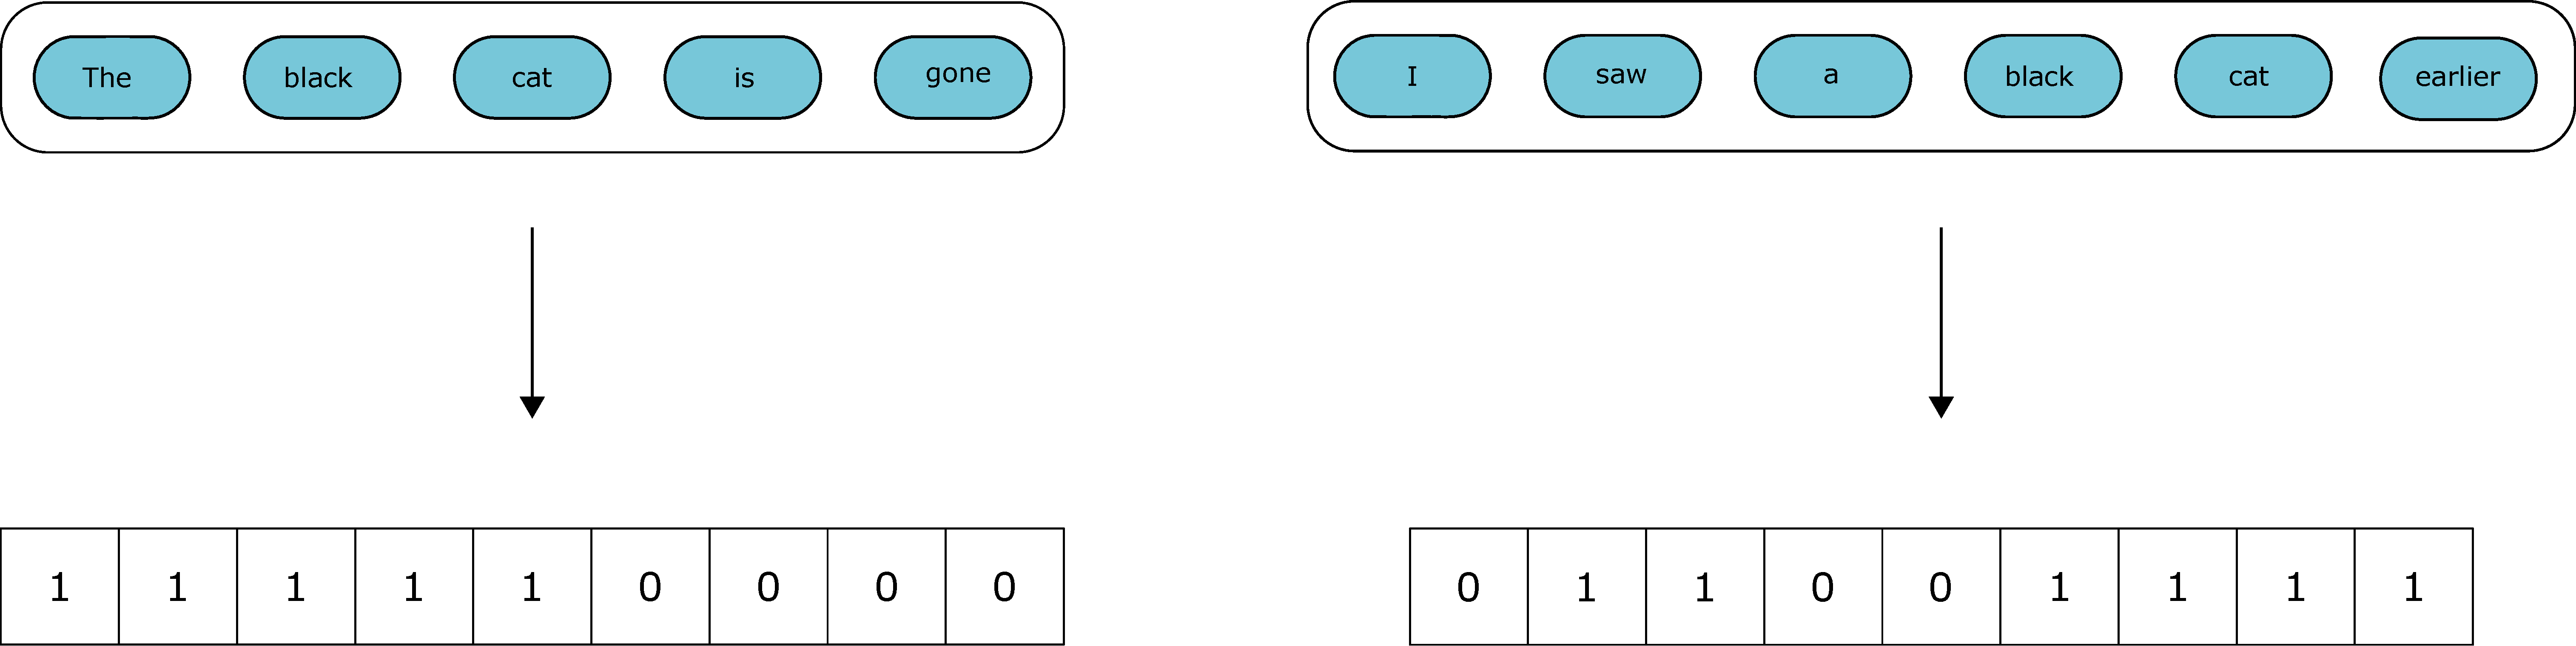
\includegraphics[width=\textwidth]{bag-of-words.pdf}
    \caption{A bag-of-words representation of the documents in the toy corpus.}
    \label{fig:bag-of-words}
\end{figure}



If the corpus is larger, it is obvious that this vector would be very large since it needs to contain one element for each unique word in the corpus. It is also generally a sparse vector. Most values are zero since most of the words in corpus are unlikely to be in each document. If instead of simply putting the values to zeroes or one in the vector but the number of occurrences of each word in the document, we have arrived at a term frequency approach.

 To achieve the inverse document frequency part of the features, every word is weighted by its inverse frequency according to Equation \ref{ekv:tf-idf}. $t$ is a term present in a corpus $D$ and $D_t$ means a document containing  term $t$. This formula ensures that common words prevalent in many documents are granted low scores and that low frequency words that might be more informative are granted higher scores. In the above example, the words ``black'' and ``cat'' are less useful in giving information about the differences in the sentences and will be given smaller weights.

\begin{equation}
    IDF(t, D) = \log{\frac{|D|}{|D_t|}}
    \label{ekv:tf-idf}
\end{equation}

Putting together the word-of-bag, term frequency and inverse document frequency approaches, each document is represented by an $n$-dimensional vector, where the coordinates are TF-IDF weights of the document. Similar documents will have similar coordinates in this vector space and will thus be closer to each other in the coordinate system. It is thus quite intuitive how this approach can be used to create feature to separate classes of documents.


 There are two downsides to this approach: 
 \begin{enumerate}
 \item  The biggest one is that the context of the words is lost. The order of words can drastically change the meaning of a sentence and is often crucial to figure out if a comment is toxic or not. The TF-IDF approach, however, has no way to model the structure of the sequence and this type of understanding of human language is completely left out of the method.
 \item  The other downside is how sparse the vector is. For very large corpora, there can be millions of unique words with most not present in any one document. This is computationally inefficient and can potentially cause memory problems. This can be solved by limiting the vector to a certain size and selecting what words should be included by some sort of heuristic, such as the number of appearances. Limiting the length of the vector will however cause some information from the documents to be lost.
 \end{enumerate}

\subsection{Bidirectional Long Short-term Memory}

\emph{Long short-term memory} (LSTM) is a special class of artificial neural networks. Instead of working on single data points, where the order does not matter, LSTM models work on sequences of data. To handle dependencies in the sequences, they have then the ability to remember earlier data points indefinitely \citep{971021502119971115}. Later on, a special \emph{forget gate} was added to also give the ability to forget all earlier activations at certain points and reset the hidden state of the node \citep{gers1999learning}. There are many small variations of LSTM, but the key points are the following:

\begin{itemize}
    \item A \emph{cell} remembers the earlier state of the node and passes it on to the next node;
    \item An \emph{output gate} sends out an activation value based on the hidden value and the input value;
    \item A \emph{forget gate} decides which part of the hidden state to forget based on the input;
    \item An \emph{update gate} decides which part of the hidden state to update and how based on the input.
\end{itemize}

\begin{figure}[ht]
    \centering
    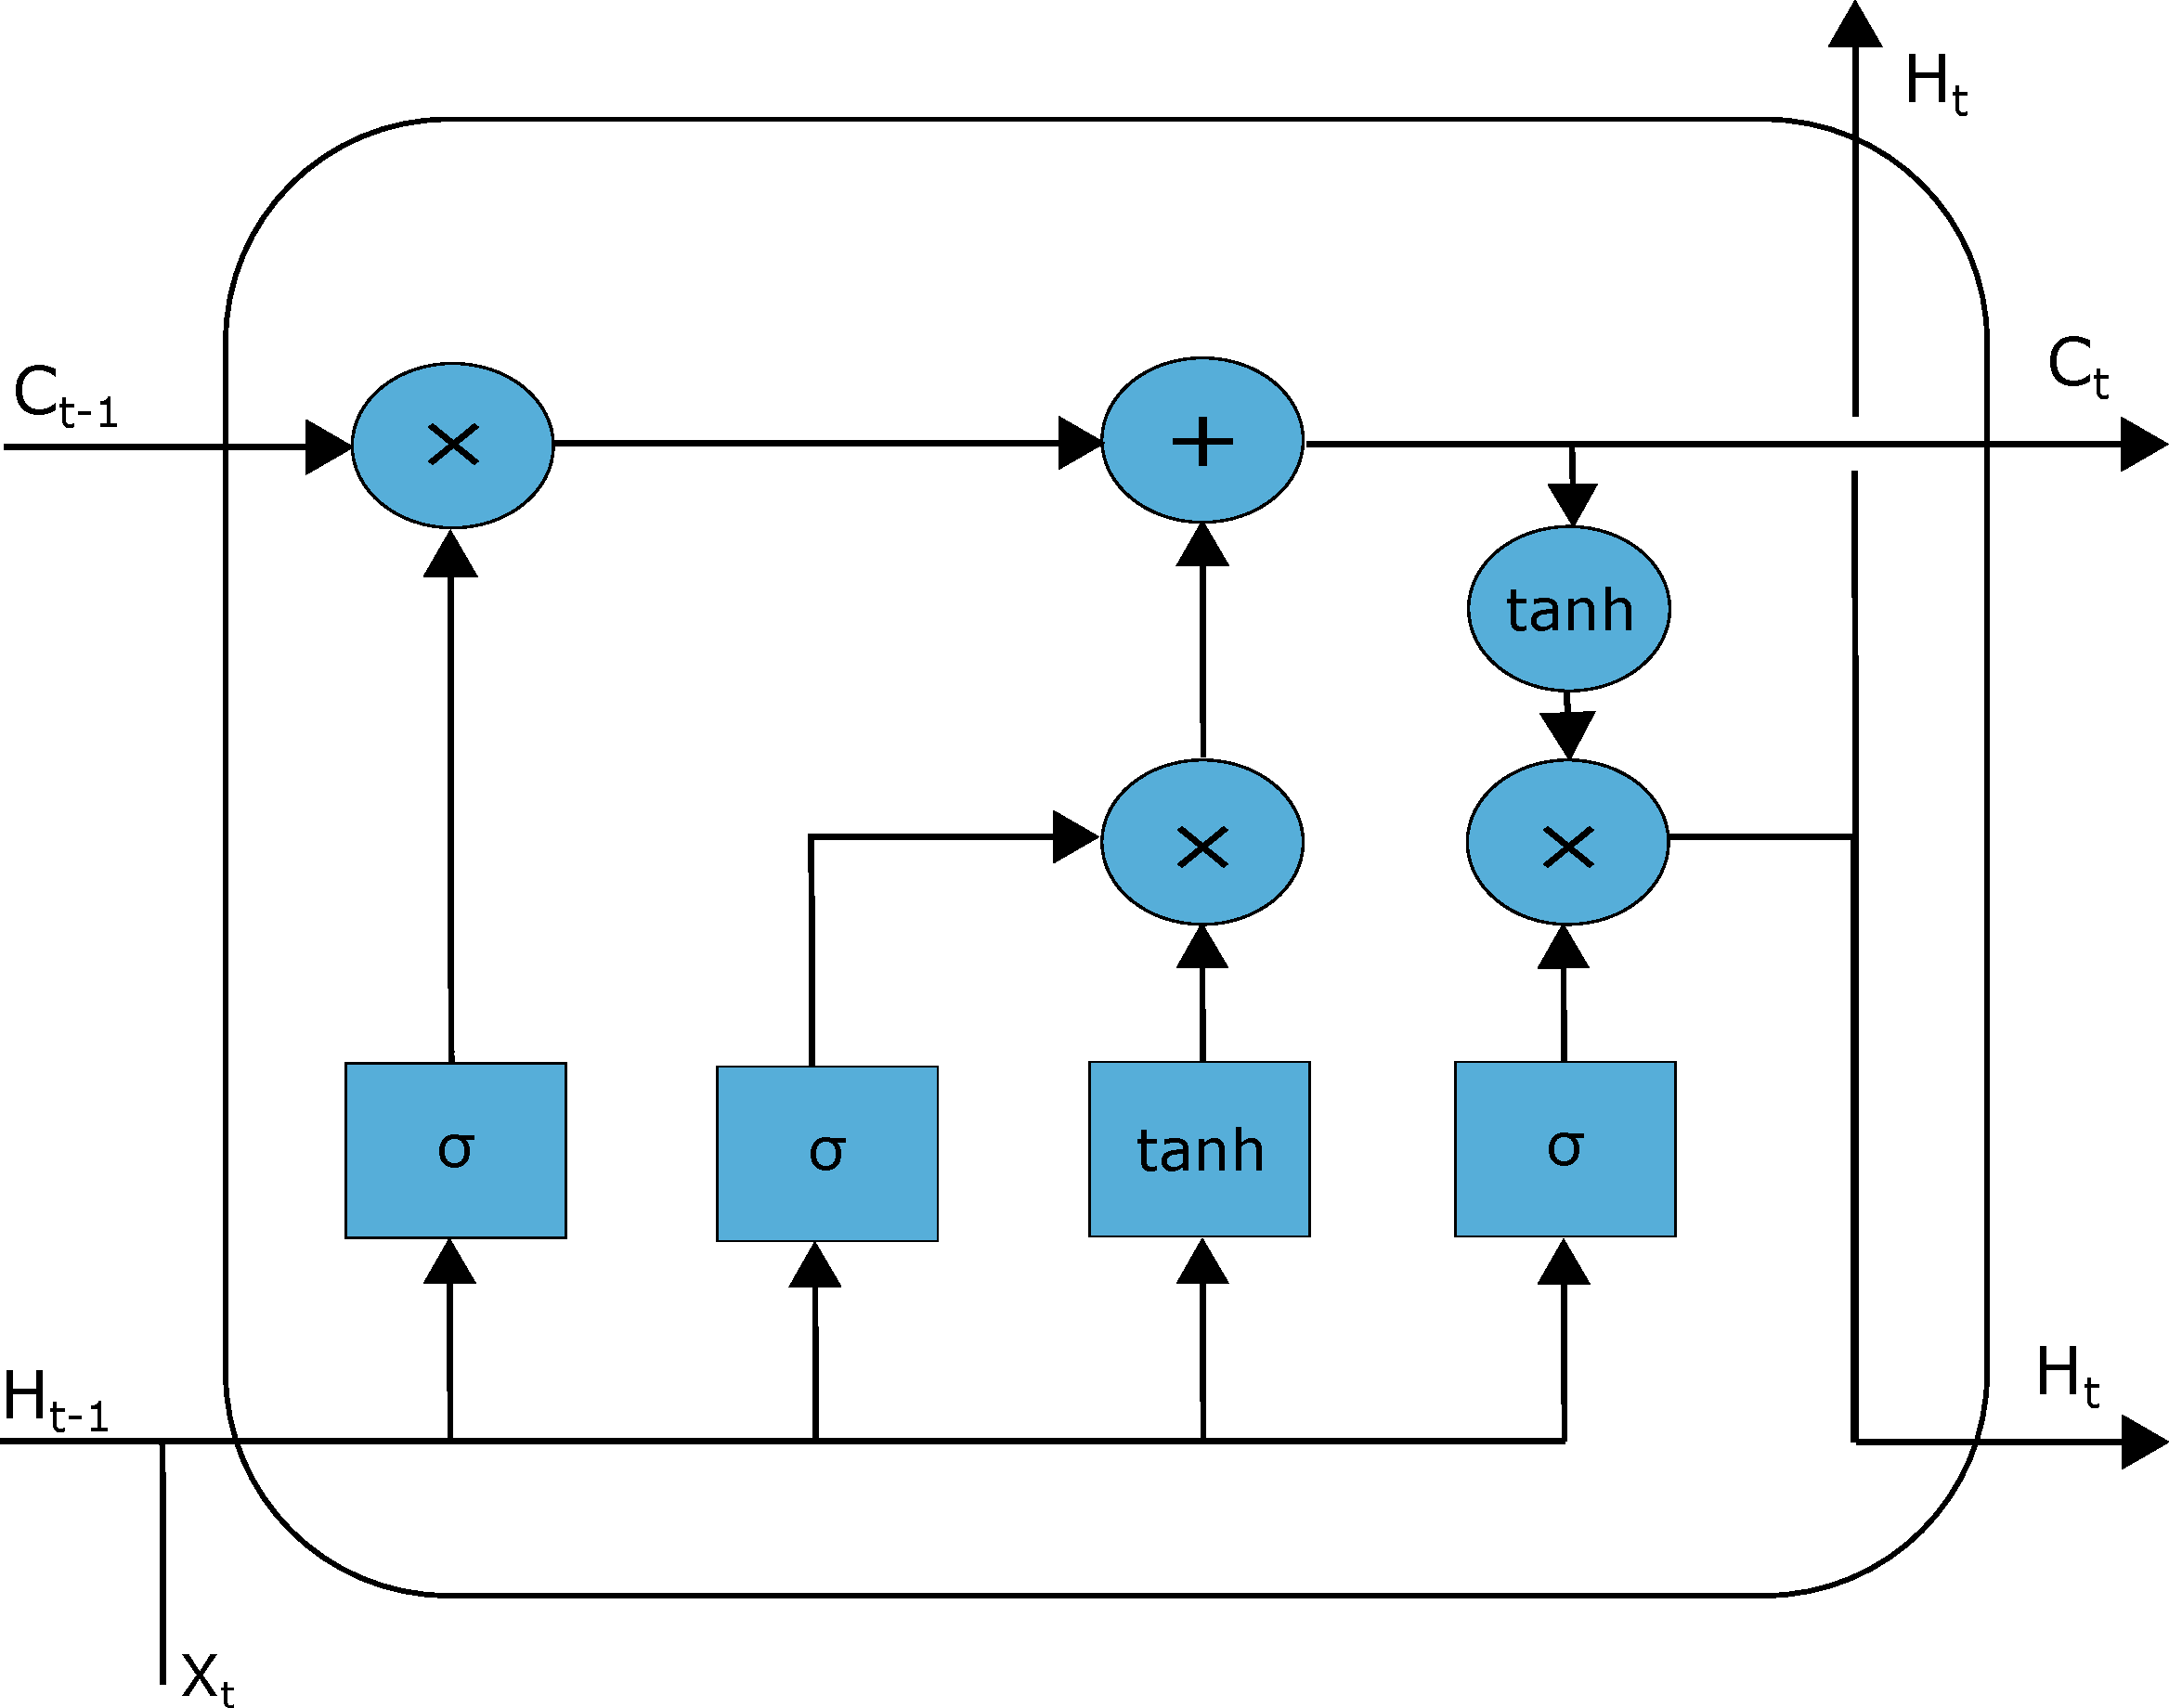
\includegraphics[width=\textwidth]{LSTMnode.pdf}
    \caption{An LSTM node.}
    \label{fig:LSTMnode}
\end{figure}

Figure \ref{fig:LSTMnode} shows the unidirectional implementation from \citet{gers1999learning}. In Figure \ref{fig:LSTMnode}, the rectangles are neural network layers and the circles are pointwise operations.  $\sigma$ represents the sigmoid function, $\tanh$ the hyperbolic tangent function, $\times$ multiplication and $+$ addition. Two lines joining into one means a concatenation and one line splitting in two means copying. $C_t$ is the cell's hidden state at time $t$ and likewise, $H_t$ is the output value and $X_t$ is the input value at the same time. $H_{t-1}$ and $C_{t-1}$ are, respectively, the output value and the hidden state from the prior data point in the sequence. The most important part in this figure is the almost straight line between $C_{t-1}$ and $C_{t}$. Unless the first sigmoid layer has a very low activation value, most of the value in the hidden state will be passed on to the next data point in the sequence after being updated in the next step.

This sequence does not have to depend on relations in only one direction. As \citet{graves2005framewise} showed, this can be applied to both the sequence fed forward and the sequence fed backward. 

The ability to model sequences of words and put them in context makes it possible for the bidirectional LSTM models to make conclusions that can't be drawn from unordered text data. This opens up new potentials in discovering hateful speech that simple statistical methods like TF-IDF cannot catch. Potentially, they can understand what words are negated in a sentence and the targets of the words.

\paragraph{Word and character embeddings.}
So far, I have not described how the words are represented mathematically inside the LSTM model. The most common approach, and the one used in this thesis, is dense high-dimensional vectors. Usually these vectors are pre-trained on large unannotated corpora to make similar words have similar values. Skip-gram methods \citep{mikolov2013efficient} are among the most popular ones for this, where words that appear in similar contexts have similar values. In this thesis, I used  a variation of skip-grams called fasttext embeddings \citep{bojanowski2017enriching}, that takes subword information into account during the pre-training.

To these word embeddings I added a second component. Inspired by \citet{DBLP:journals/corr/ChiuN15}, every word is divided into its constituent characters and these are then represented by embeddings. The character embeddings are trained at the same time as the text classification task. On these embeddings, the spatially close characters in the same word are fed to a convolutional neural network together. The results are maxpooled, flattened, and then concatenated to the word embeddings before being passed to the LSTM nodes of the network. 

With this added information, the model has the ability to still use information from words not seen during training. It is then more robust to spelling errors. Figure \ref{fig:bilstmmodel} shows how the resulting model looks like. Importantly, the activations from the character convolutions are synchronized with the word embeddings when they are input to the LSTM nodes.

\begin{figure}[ht]
    \centering
    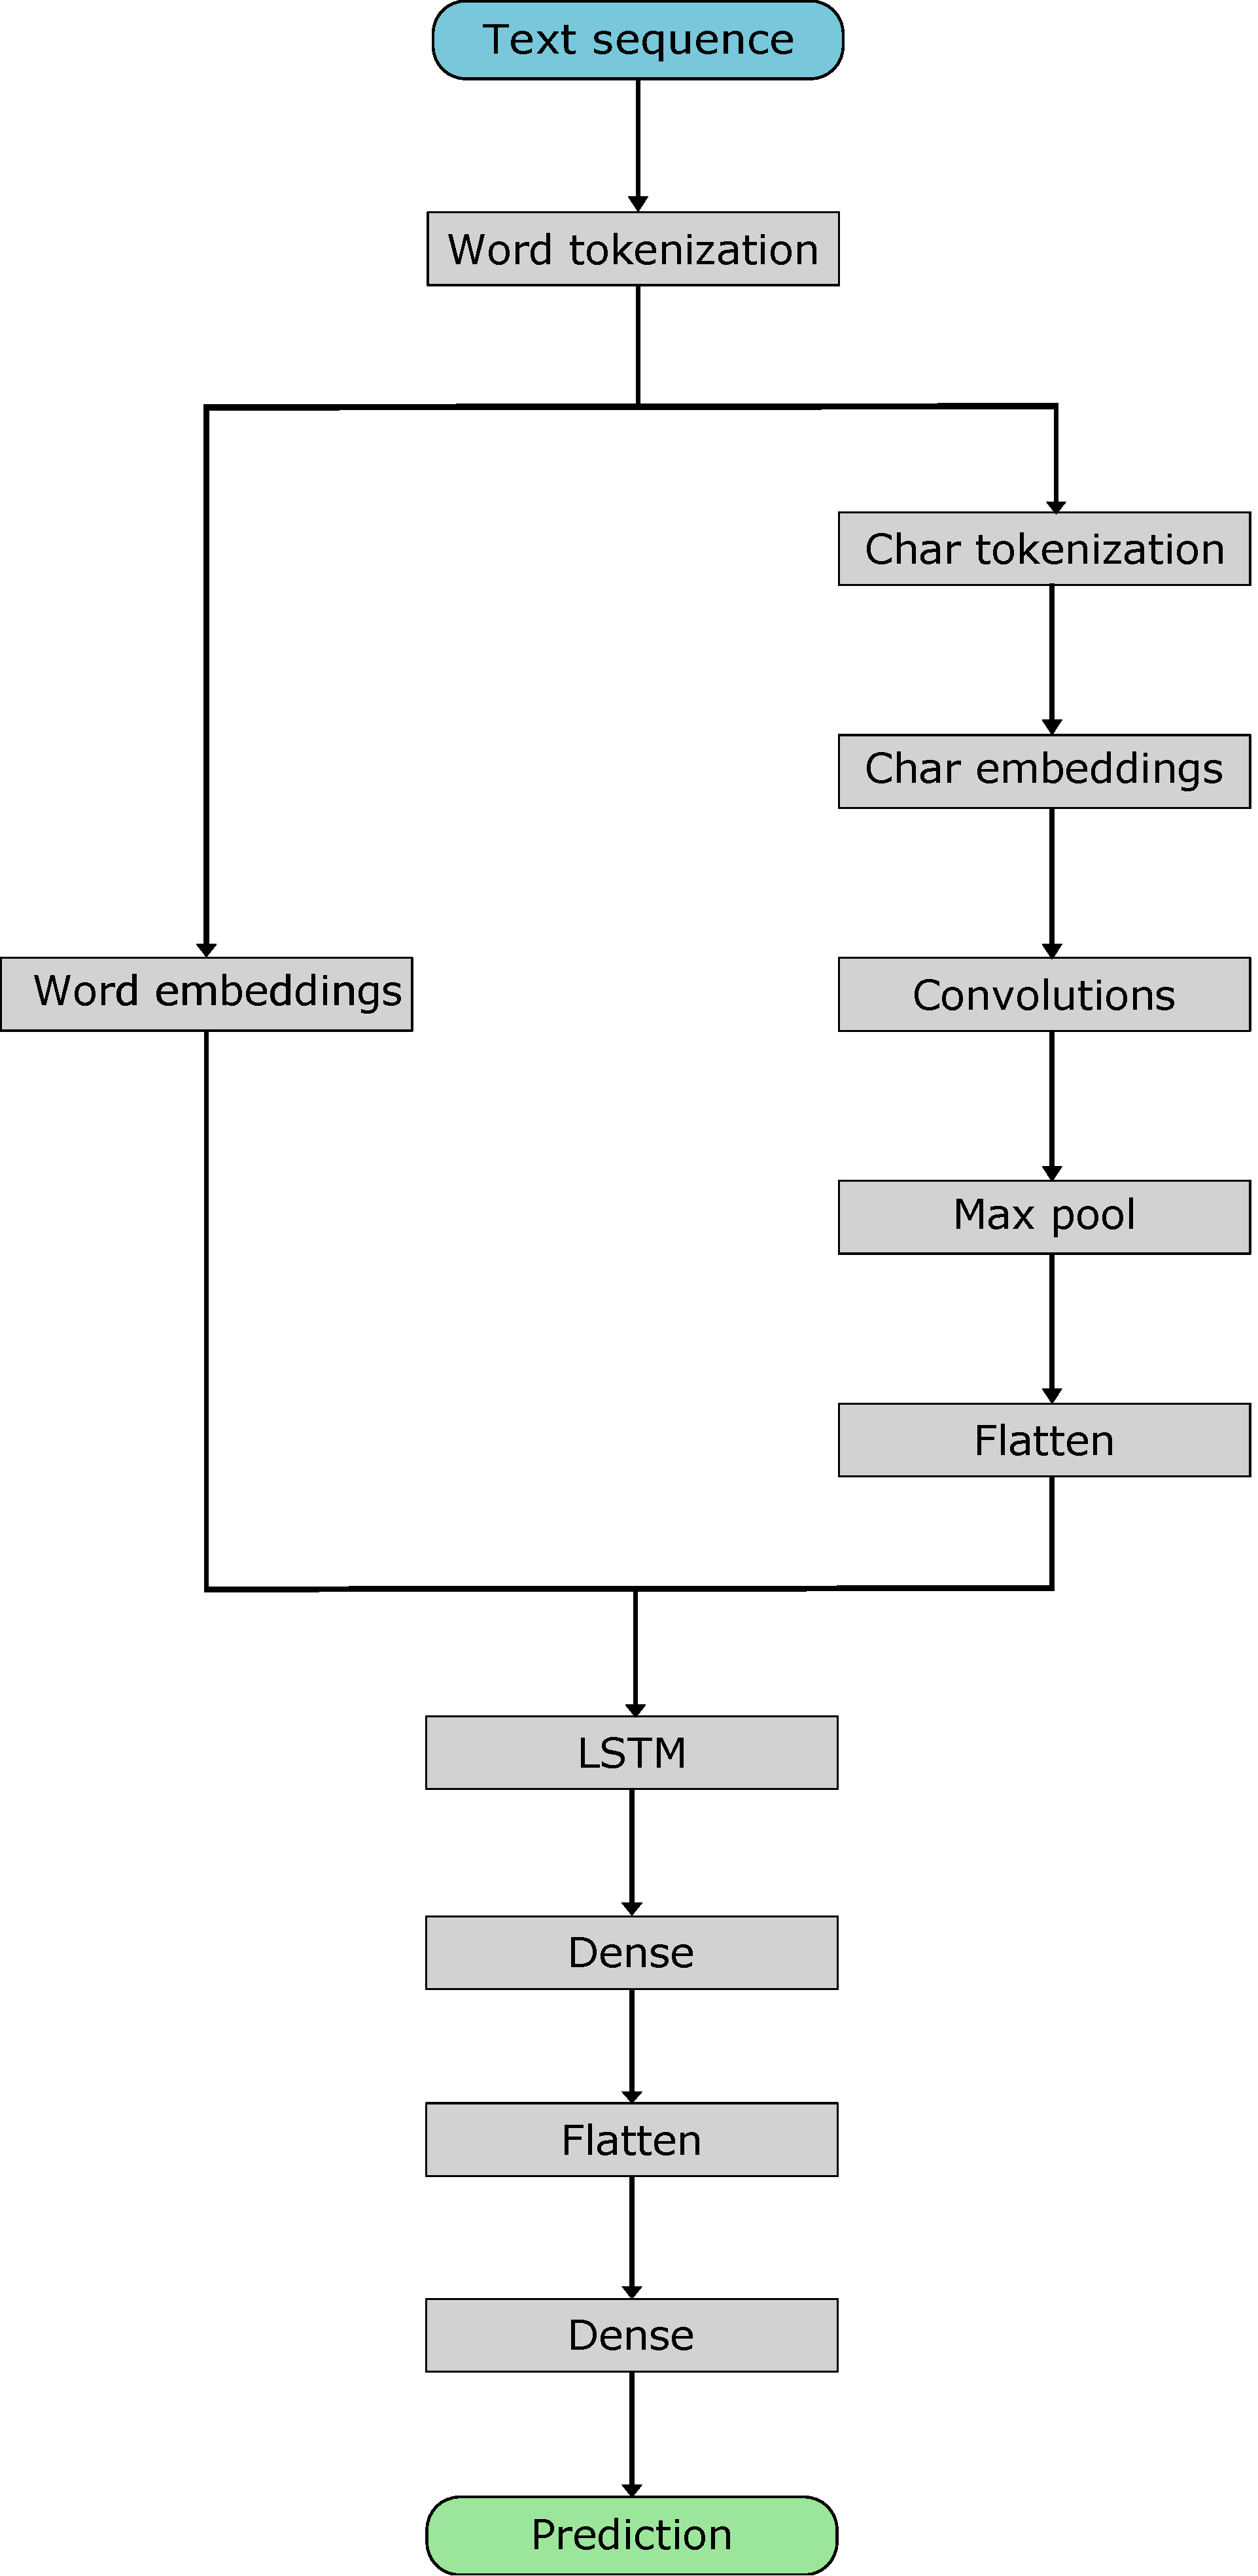
\includegraphics[width=\textwidth*2/3]{BiLSTM.pdf}
    \caption{The BiLSTM model with character convolutions.}
    \label{fig:bilstmmodel}
\end{figure}


\subsection{Transformers}

Transformers are currently at the forefront of natural language processing and are being improved continuously with, for example, architectures such as XLnet \citep{DBLP:journals/corr/abs-1906-08237}, RoBERTa \citep{DBLP:journals/corr/abs-1907-11692} and of course the Bidirectional Encoder Representations from Transformers (BERT)  \citep{DBLP:journals/corr/abs-1810-04805}, all being less than two years old at the time of writing. 

Compared to other techniques, they add another step towards understanding context in text and they do this with effective large-scale pre-training. Transformer models pre-train a language model on unannotated corpora. To accomplish downstream tasks, such as classification, they add an output layer for the task. The model with the new output layer is then finetuned on a smaller set of data. For text classification this means a dense layer with softmax activation.

Transformers are effectively a form of transfer learning, where the knowledge gained from the unannotated corpus improves performance in tasks not directly related to it. While there were forms of transfer learning before, transformers quickly proved to be more effective. The first of them, BERT, when published, achieved state-of-the-art results in several different tasks \citep{DBLP:journals/corr/abs-1810-04805}.

The key to these better results are the way the training can model human language better than earlier attempts and effectively learn from larger corpora than earlier models. The training for BERT consisted of two steps:
\begin{enumerate}
    \item Prediction of masked tokens in a sentence.
    \item  Next sentence prediction.
\end{enumerate}

To exemplify this, I will use another toy corpus. Take the two sentences:
\begin{quote}
There was a black cat. It walked over the street.
\end{quote}
In the masked word prediction during training, the model will mask 15\% of tokens. Figure \ref{fig:BERTmasking} shows a possible result for the first sentence. The BERT model will try to predict the masked token and, if wrong, penalize the prediction.

\begin{figure}[ht]
    \centering
    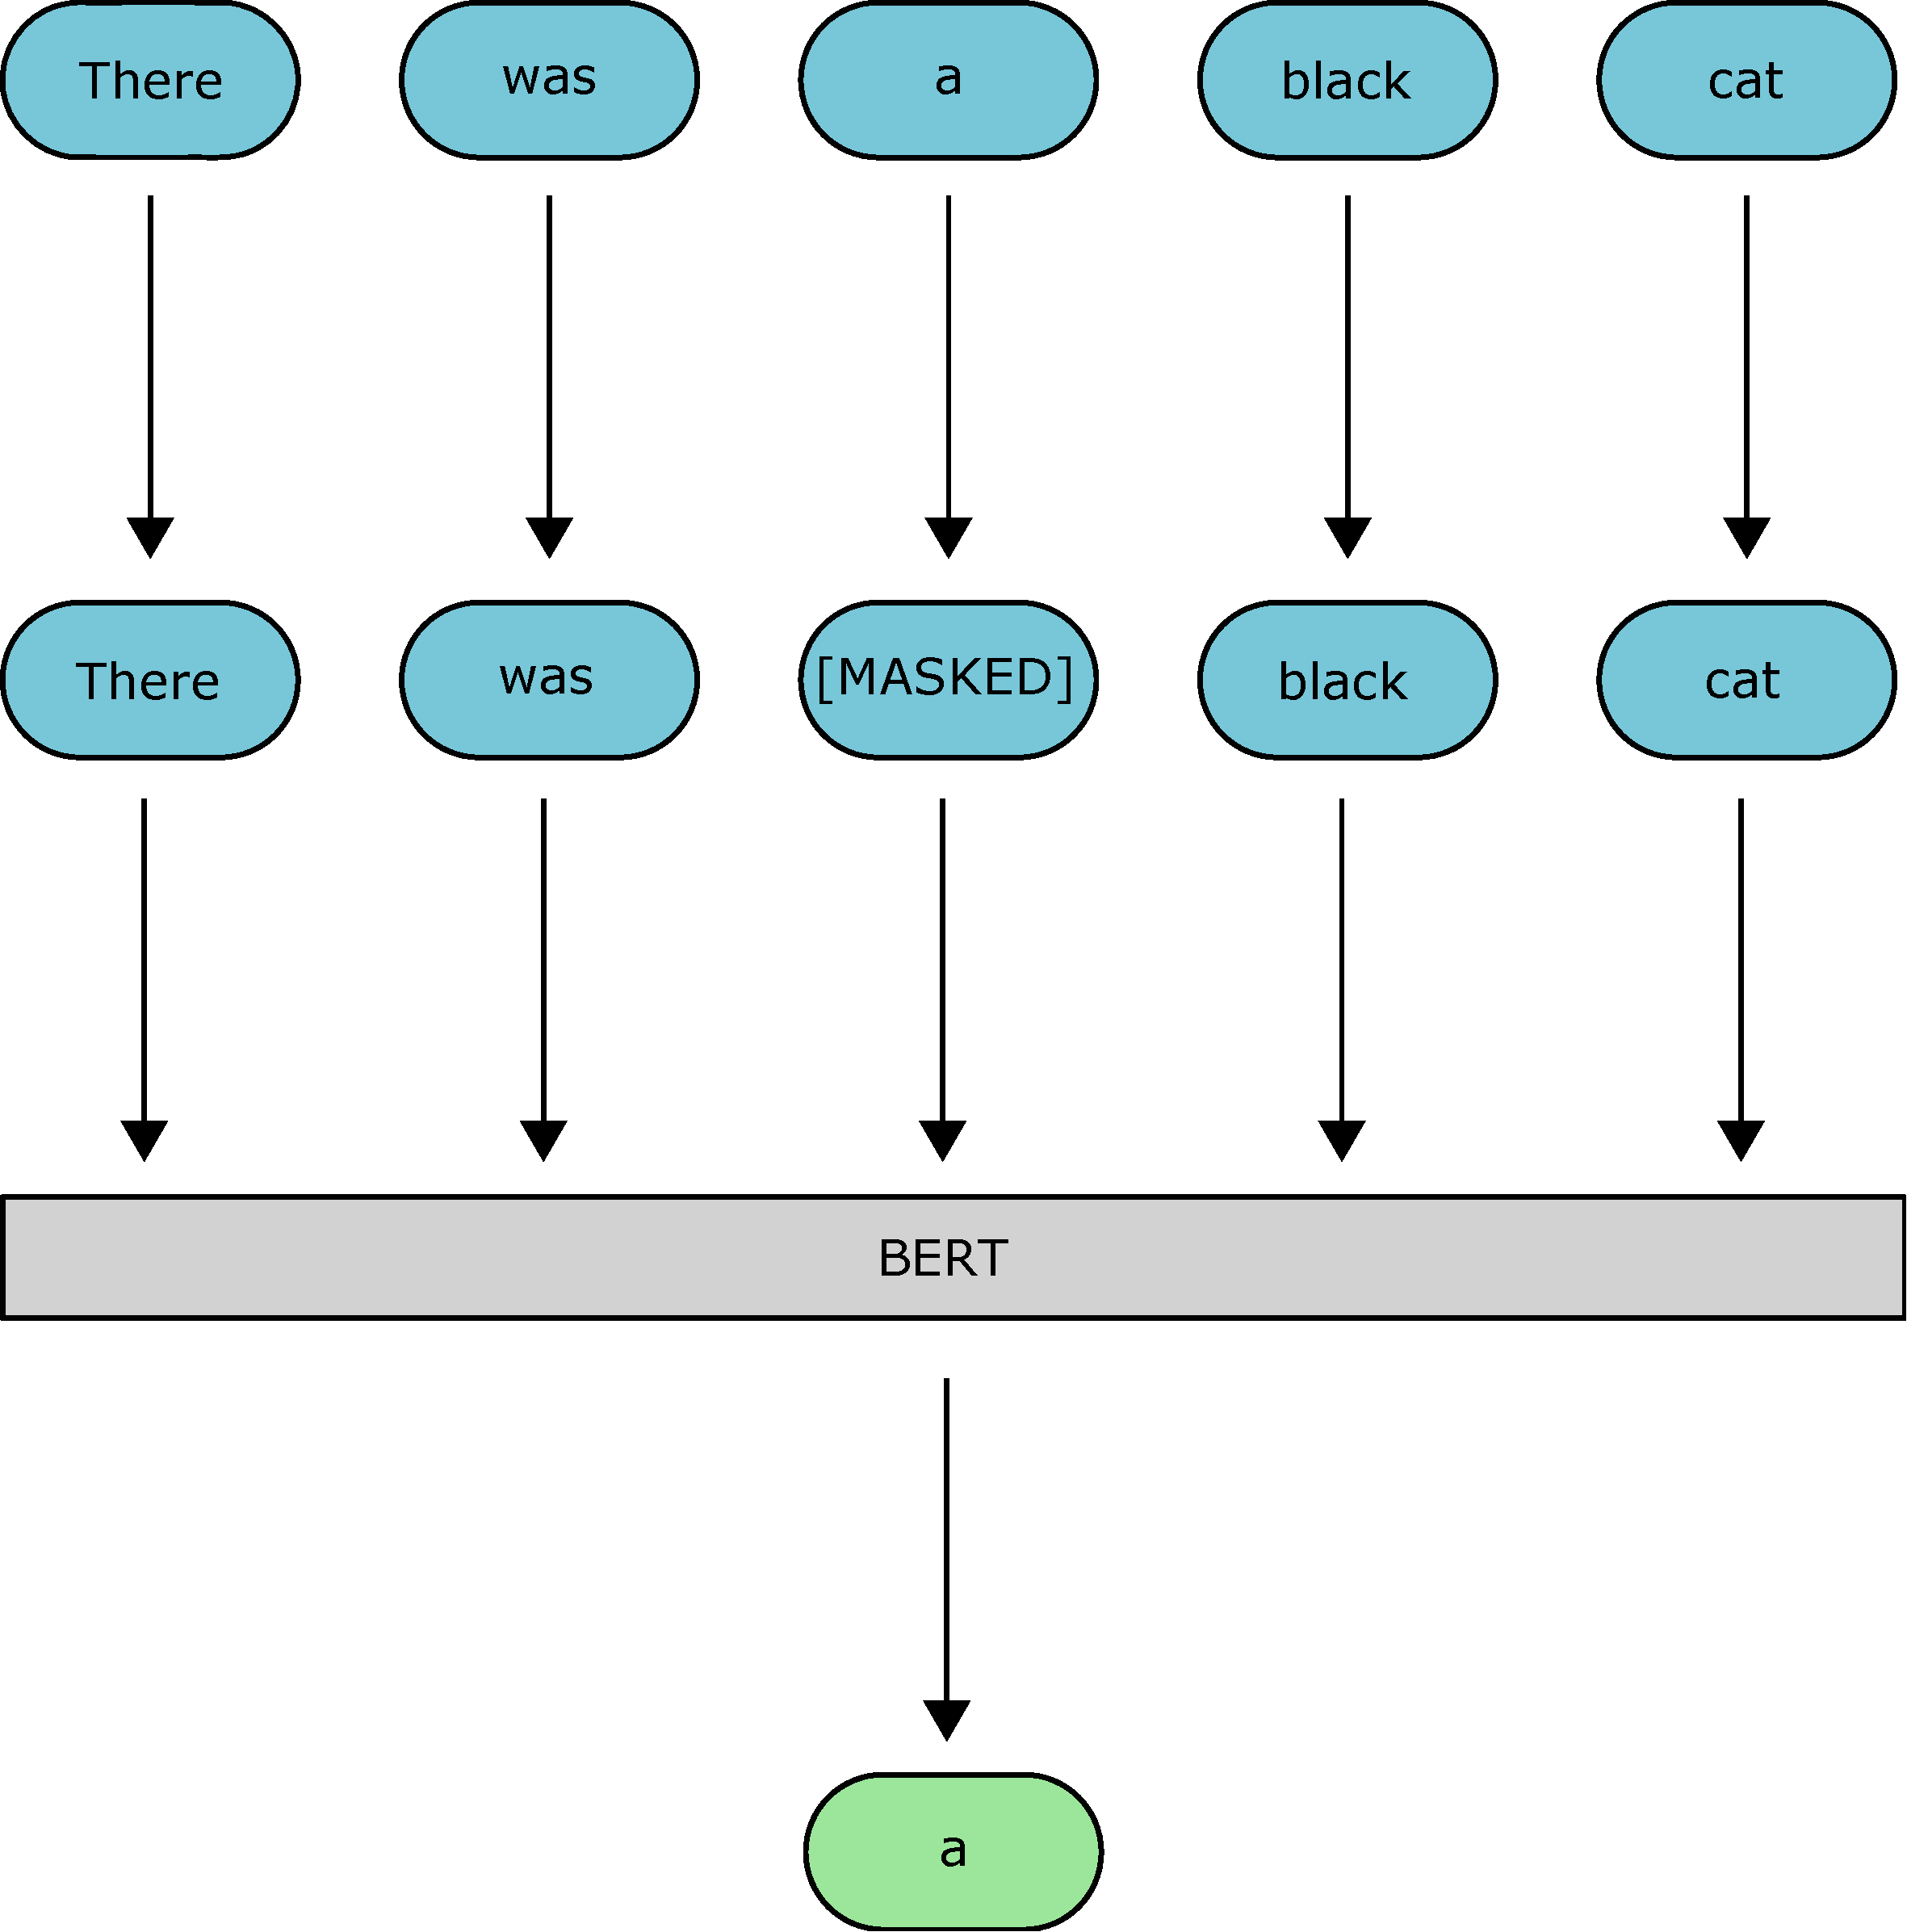
\includegraphics[width=\textwidth/2]{BERTmasking.pdf}
    \caption{An example of BERT masking and word-level prediction, often called masked language modeling.}
    \label{fig:BERTmasking}
\end{figure}

The next training goal requires the training corpus to be ordered. Given a sentence $A$, a sentence $B$ is chosen, with 50\% probability either being the following sentence from the corpus or, with 50\% probability, a random sentence from the corpus. The prediction the model determines if the sentence $B$ is or isn't the next sentence in the corpus. 

These two goals make up the pre-training process of BERT.

While the upside of state-of-the-art results is clear, there is a downside. To accomplish its goal BERT has an immense computational cost for this pre-training. For example, \citet{DBLP:journals/corr/abs-1906-08237} state that they spent several days pre-training with large computational capacity:

\begin{quote}
Specifically, we train on 512 TPU v3 chips for 500K steps with an Adam weight decay optimizer, linear learning rate decay, and a batch size of 8192, which takes about 5.5 days. It was observed that the model still underfits the data at the end of training.
\end{quote}

This will clearly prove a problem if quick iterations are needed and makes it unpractical to pre-train transformer models. Luckily, for most languages, these models are already available from research institutes or private companies on platforms such as the HuggingFace library \citep{Wolf2019HuggingFacesTS}.

\paragraph{Cross-lingual transfer learning with transformers.}
Just as transformer models revolutionized transfer learning in natural language processing at large, they also have revolutionized transfer learning between languages. As \citet{DBLP:journals/corr/abs-1901-07291} showed, effective cross-lingual models can be trained. If parallel corpora exist, the model can even utilize resources in other languages in the language model pre-training. These techniques, once again, greatly improved state-of-the-art performance on several tasks, this time with multilingual objectives. Most interestingly for the goal of this thesis, \citeauthor{DBLP:journals/corr/abs-1901-07291}  report state-of-the-art performance on the XNLI data, where the tasks are cross-lingual and zero-shot, i.e. learning to accomplish different tasks with only labeled data in another language than the target language \citep{DBLP:journals/corr/abs-1809-05053}.

Once again, the training process is in theory not very complex. XLM shares BERT's training goal of masked language modeling shown in Figure \ref{fig:BERTmasking}, but also causal language modeling, i.e. given a sequence of words, predict what word will follow.

The cross-lingual training is what they named \emph{translation language modeling}: Given two identical sentences in different languages, mask 15\% of tokens randomly and use the sentence in both languages to predict the missing tokens with cross-lingual connections. Figure \ref{fig:TLM} shows an example of this.

\begin{figure}[ht]
    \centering
    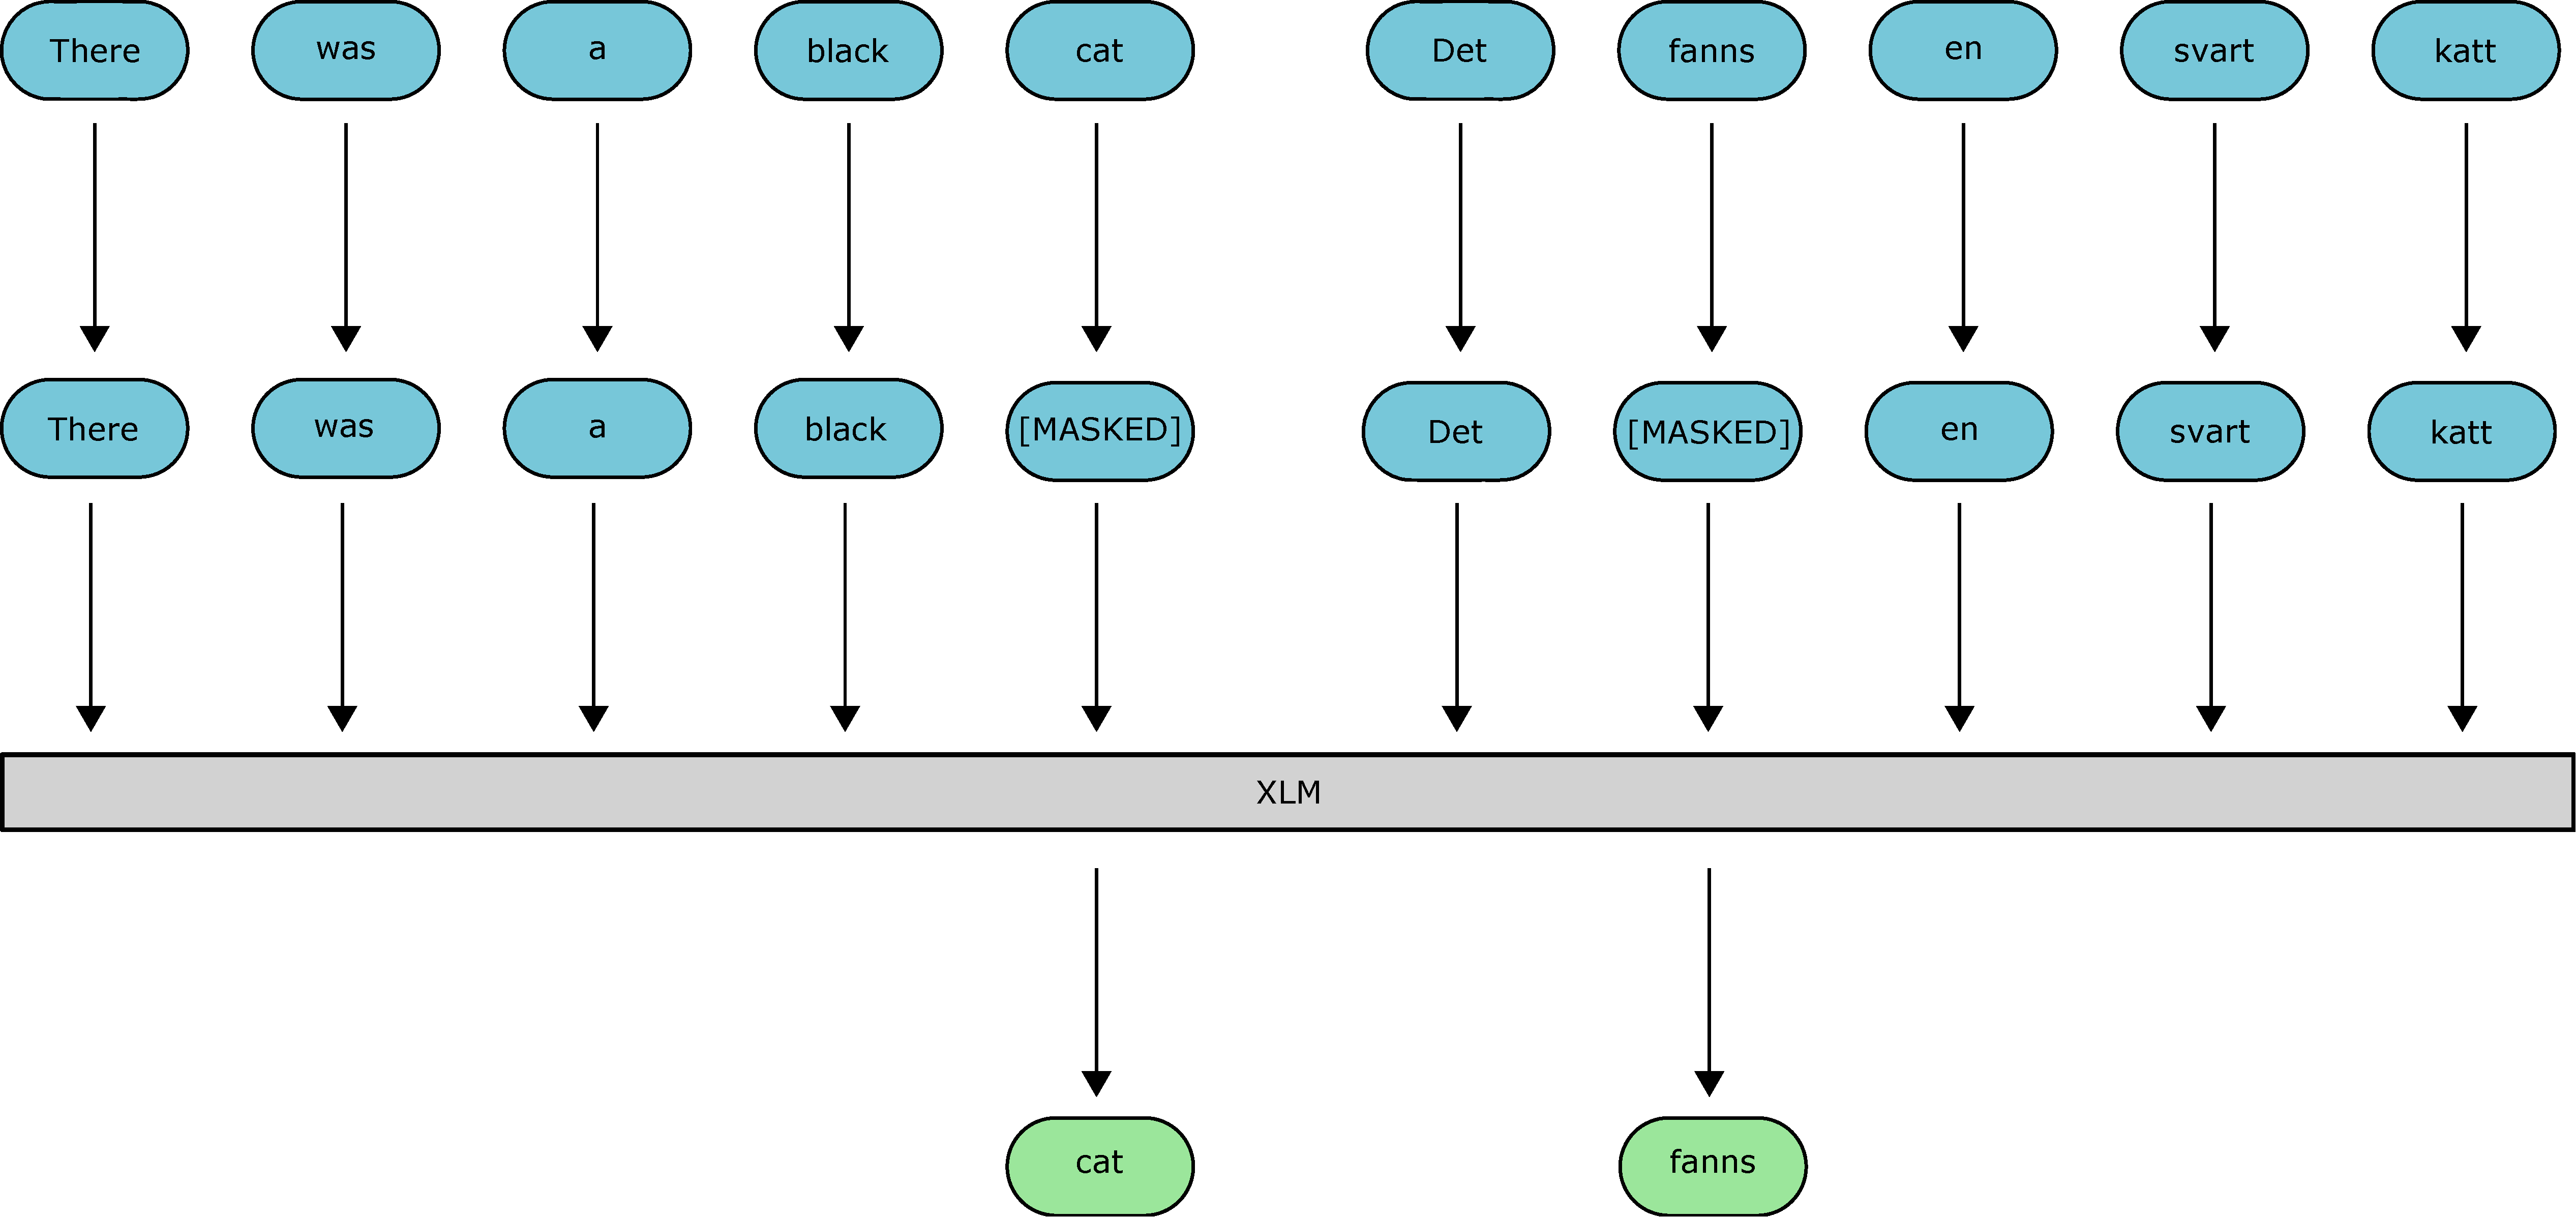
\includegraphics[width=\textwidth]{LTMmasking.pdf}
    \caption{An example of translation language modeling.}
    \label{fig:TLM}
\end{figure}

During training, the model will learn to translate between languages and what words are similar. The model can learn both to understand the context in one language, but also gain understanding by comparing the sentence to the same sentence in another language. The success of their approach on several benchmarks proved that similar methods used by \citet{DBLP:journals/corr/abs-1810-04805} to model context between words can also understand similarities between languages.

%Learning from other languages is often studied because it means that data for one language can be used for another language where such resources might not be available. Doing this means that low resource languages can be equalized in some sense to other more high resource languages such as English or in the case of Ifrågasätt, Swedish. If the data generated in Swedish can be used for other languages the ease of Ifrågasätt expanding to other countries is decreased dramatically. (Det här borde uppenbarligen stå i introduktion)

%There are several methods to achieve this result. But first it might be useful to not even attempt transfer learning. How easy is it to expand to another country without any training or validation data at all? (Inte säker om det här ens är värt att testa. Man kan använda kända listor över hatiska ord t.ex.)

%Using transfer learning from Swedish makes us ask how one would transfer the knowledge in one language to knowledge in another. This can be seen as us having have two input domains, Swedish and a foreign language. We have a model for the Swedish language that maps it to our output vector, ``Toxic'' or ``Not toxic''. Our task is to somehow make this model doing calculations on the domain of Swedish work on another domain, the foreign language. To use transfer learning in this essay ultimately two different approaches will be used. The first of these is to map the foreign domain to Swedish domain, i.e. add a first step that translates the foreign language to swedish and then uses the old model. 

%The second one aligns the two domains. Natural language processing problems commonly map text to dense word vectors with many dimensions as a preprocessing step before feeding these representations into a neural network. Both the foreign language as well as the Swedish language maps to these vectors, but these are not necessarily aligned. It is possible to do so using for example Facebook's MUSE %\citep{conneau2017word}.
%We can translate the Swedish data to an intermediate domain and then train the model from this intermediate domain. To evaluate in another language, we simply translate the language to the same intermediate domain and then use the model trained on the Swedish dataset.

%The more finegrained part of text classification tasked with finding offensive text or toxic comments has an earlier history in online communities. In 2019 a competition called OffensEval was held with the goal of identifying offensive tweets, how they were offensive and against what group or person \citep{zampieri2019semeval}. The competition format proves very helpful as we can not only identify the better approaches but also discard some approaches that does not prove fruitful. 

\chapter{Datasets}

This chapter describes two distinct datasets:
\begin{itemize}
    \item The first one from Ifrågasätt that is used to understand characteristics of newspaper comment data and 
    \item A second one, the OffensEval competition dataset, that is used to test cross-lingual models. 
\end{itemize} 

I will mainly focus on the Ifrågasätt dataset, describe how it was created and made usable for a classification problem. I will give some details on its characteristics that are relevant for understanding the problem of working with the data. I will present the OffensEval dataset as a reference.

\section{The Ifrågasätt data}

The primary objective of the round-the-clock human moderating at Ifrågasätt is to keep the comment section clean. It has another consequence: Every comment on the platform becomes a labeled data point. Unfortunately, this data was not created with the intention of being used to solve classification problems and is not divided into categorical classes.

The moderators work has so far resulted in all the published comments being placed in one of several classes: Visible, hidden, approved, user removed, and deleted:%Borde jag ens ha med en sådan här lista? Kanske är onödigt att förklara mer än vad "hidden" innebär.
\begin{description}
  \item[Visible] means that a moderator has taken no action for this comment and that it is visible to everyone since the comment author wrote it.
  \item[Hidden] means that the comment has been unpublished by the moderators. It is not visible on the Ifrågasätt platform, but it remains in the database.
\item[Approved] means that a moderator has verified that the comment is fit for the platform. This tag might happen when a comment gets reported by a user and the moderator clears it later or the moderators change their mind whether a comment is following the rules. 
\item[User removed] is self-explanatory: Comments can be deleted by users and these have their own status. 

\item[The removed status] is reserved for when a moderator does hard deletes of comments such as in the cases of spam or a user sending a request to delete their own comment. However, this category is not consistently used for these purposes.
\end{description}

\subsection{Generating categorical data}

Of these classes, all toxic comments are in the \emph{hidden} class. Unfortunately not all hidden comments are necessarily toxic comments. Every hidden comment has a reason for the being hidden saved in the database, stated in plain text. These reasons for deletions state what rule the comment broke that caused is to be hidden. This means that the ``hidden'' class is divided into several subclasses. Some of these finer separated classes are not necessarily problems in themselves. Insults and general racism are separate as reasons for moderators to remove the comment, but both fit the larger class of a toxic comment. 

Other reasons however, such as being off-topic or posting two identical comments are crucial to separate from toxic comments. An off-topic comment on one article might be a normal comment on another article. A comment posted twice that is civil means that there exists one copy of the comment that is deleted and one that is approved that are identical in content. These comments, while deserving to be removed from the platform, do not fit the criteria of being toxic or offensive. Due to this, they are outside the scope of this thesis and therefore have to be separated from the other hidden comments that fall under the toxic subclass.

The comments also aren't necessarily confined to one class. A comment can be all three of off-topic, toxic, and needlessly repeated. For the purposes of this thesis, if a comment belongs to more than one classes, where one is the toxic class, it is considered a toxic class.

Luckily for us, while the comments aren't strictly split into classes, the reasons for deleting comments are mostly copied and pasted from a template. Certain status messages or slight variants are used for most comment categories. These templates are key to quickly understand which comments are toxic or not.

I classified the comments into non-toxic and toxic using this algorithm:

\begin{enumerate}
    \item Remove all comments that do not have the hidden status.
    \item Remove all non-unique reasons for deletion.
    \item For every reason:
     \begin{enumerate}
         \item Read through the reason for deletion and see if the comment was removed for being hateful.
         
         \item If hateful, add the part of the reason that made it interpreted as hateful to the list of toxic templates.
     \end{enumerate}
    \item Filter out all the reasons that are already classified as hateful and repeat step 3 until no new reasons can be found.
\end{enumerate}

I applied the list of templates for saying that a comment is hateful to every comment in the database and put it into the non-toxic or toxic class for use in a classifier.

\subsection{Exploratory data analysis}

The process described in the previous section divides the Ifrågasätt dataset into two distinct classes. To gain some further understanding of the problem, I present some descriptive statistics about the data here to motivate future hyperparameter choices.


Table \ref{tab:deskriptiv} shows the majority of this information. As seen, hidden comments tend to be shorter than visible ones and the toxic comments only represent a very small portion of the comments in the dataset, where only roughly 2$\%$ are toxic. 

To get a better view of the comment length, see Figure \ref{fig:distribution} and the peak at comment lengths around 150 characters. Comments that are longer than 1500 characters cannot at this time be published on the platform. This explains the second peak at the tail of the distribution.

\begin{figure}[t]
    \centering
    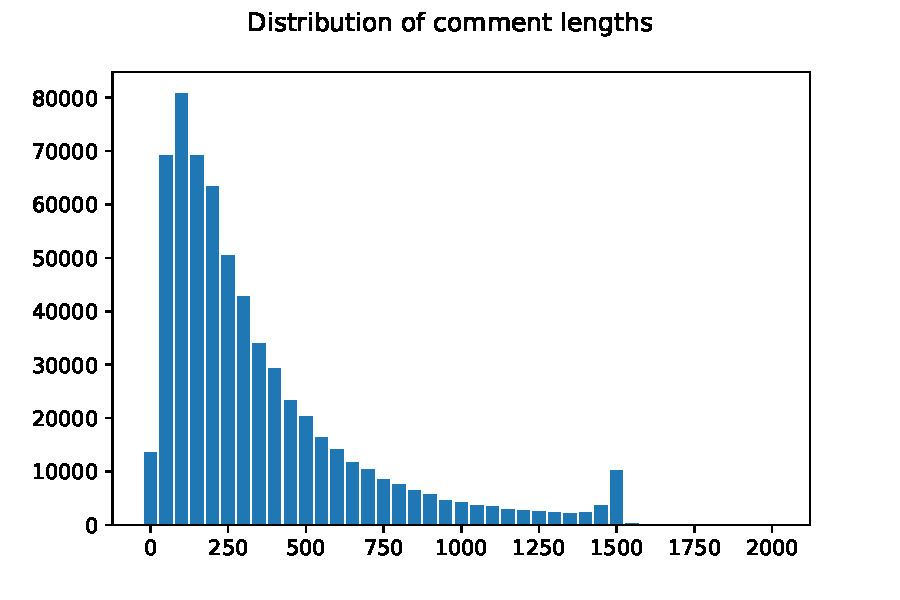
\includegraphics{langddistribution.pdf}
    \caption{Distribution of comment lengths in characters rounded to the closest factor of 50. Y-axis is frequency and X-axis is comment length.}
    \label{fig:distribution}
\end{figure}

\begin{table}[t]
\centering
\begin{tabular}{@{}lrrrrr@{}}
\toprule
Category    & Number of comments & Mean & Standard deviation & Max   & Min \\ \midrule
All classes & 719,217 & 179  & 177                & 15,378 & 1   \\
Toxic       & 11,347 & 158  & 166                & 3,007  & 5   \\ 
Non-toxic   & 707.870 & 180 & 176 & 15,378 & 1 \\\bottomrule
\end{tabular}
\caption{Descriptive statistics about some classes in the Ifrågasätt dataset.}
\label{tab:deskriptiv}
\end{table}

\subsection{Analyzing the annotation at Ifrågasätt}

Reliable, consistent annotations between two annotators and one annotator at different times is essential to a good moderation. It also means that guidelines for a task are clear and that different annotators understand them similarly and act similarly after reading them. This will lead to a large inter-annotator agreement, which in turn will show that information in the data points can be used to reliably determine the category. 

However, if there is a low inter-annotator agreement, this clearly poses a problem for a classification task. If two annotators often disagree on how to annotate the same or similar data points, this means there are discrepancies with how they assign categories. This shows that either the task is not well-defined or that the annotators have failed to understand them the same way due to issues with training. For a classifier, the maximum possible performance is a function of both the difficulty of the problem but also the quality of the data that has been generated. It is therefore possible that the low performance of the dataset is not only a result of the higher difficulty of the problem, but also the annotation.

For these reasons, I investigated the inter-annotator agreement of the Ifrågasätt dataset. Two moderators working at Ifrågasätt received each 95 different comments to annotate. Half of these comments had been annotated earlier as offensive and half of them as non-offensive comments by the moderator team. Ideally a completely random sample from the corpus should have been drawn but due to the heavy class imbalance and the limited time of the moderators, this was not done. Table \ref{tab:interannotatoragreement} shows the agreement results with the Cohen's $\kappa$, Krippendorff's $\alpha$, and PABAK values. Some other offensive text and hate speech corpora are included for comparisons.

\begin{table}[t]
\centering
\begin{tabular}{@{}lllll@{}}
\toprule
Datset & Category  & $\kappa$ & $\alpha$ & PABAK \\ \midrule
Ifrågasätt & All  &  0.52 & -0.04 & 0.56 \\
Ifrågasätt & Non-offensive  & 0.56 & -0.01 & 0.80  \\
Ifrågasätt & Offensive  & 0.31 & 0.00 & 0.27  \\
Turkish OffensEvak & All  & 0.72 & - & - \\
IWG hate speech & All  & - & 0.18-0.29 & - \\
Gab hate corpus & Offensive & 0.23-0.3 & - & 0.67-0.97 \\
\bottomrule
\end{tabular}
\caption{Results of two moderators annotating the same 95 comments alongside some public hate speech and offensive texts corpora. Inter-annotator agreement for the Turkish OffensEval was measured by \citet{turkoffensive}. For the IGW corpus, several different groups of annotators were measured against each other which is why a range of categories are given \citep{DBLP:journals/corr/RossRCCKW17}. For the Gab corpus, the scores were calculated on a per category basis, all of them being hate speech in some sense \citep{kennedy_atari}.}
\label{tab:interannotatoragreement}
\end{table}


The moderators described the task as harder than their normal annotation. Not knowing the source article, where the comment was posted or what comment replied to it made the annotation decision more difficult. They also mentioned that different newspapers have different criteria for what a good comment is and that these criteria  can also vary in time. Therefore the text of the comment only is not enough information to decide whether a comment is offensive or not according to the labeling standard at Ifrågasätt. 

Furthermore, the annotation task is also slightly different than the one they do in practice. I asked the moderators to flag comments that they think should be removed. They weren't asked to state the specific reason for doing so which they do in their usual work. This might lead to a slight overstatement of agreement. On the other hand, the criteria defined in the dataset chapter are quite broad and are likely to classify most comments which are removed due to offensiveness. Even if the finegrained annotations are worse, the broader categories the model is trained on will be classified similarly. Given these circumstances the values in Table \ref{tab:interannotatoragreement} are probably an underestimation of the inter-annotator agreement of the Ifrågasätt moderators. The fact the comments sampled in the investigation might also be harder than a random sample due to the selection process makes this argument stronger. It is not possible to know how misrepresentative this analysis is without repeating the investigation with a large representative sample from the corpus being drawn.

The results are as they stand: Poor compared to other corpora. The $\kappa$ is lower than the Turkish OffensEval values and higher than the Gab hate corpus, but one has to take into consideration the different prevalence between the classes. A lower prevalence of some classes decreases the $\kappa$ score even if the same amount of mistakes relative to prevalence of the classes is made \citep{byrt1993bias}. The Turkish OffensEval data therefore actually has a much higher agreement rate than the dataset the annotators at Ifrågasätt were measured with. 

This means that the other two measurements are easier to compare datasets with. PABAK was created specifically to have score that was similar to Cohen's $\kappa$, but was easier to use for comparisons between datasets \citep{byrt1993bias} But as can be seen, the dataset does not fare well in those measurements as well. As \citet{krippendorff2011computing} says, an $\alpha = 0$ means that the annotators cannot differ categories from each other better than chance itself. For the Ifrågasätt sample $\alpha$ is below  $0$. This should be interpreted as there being systematic errors that are worse than random chance \citep{krippendorff2011computing}. The PABAK value is also not much higher than the Cohen's $\kappa$ value due to the classes being relatively balanced in the sample and significantly lower than the values for the Gab hate corpus.

But it should be mentioned that all the datasets have relatively low inter-annotator agreement. The inter-annotator agreement measurements are all bounded by 1 in which case there is perfect agreement. As can be seen in Table \ref{tab:interannotatoragreement}, most datasets are far from this. The ``call to violence'' category in the Gab hate corpus comes close with a PABAK value of 0.97, but the ``offensive language'' category at 0.79 and 
``assault on human dignity'' category at 0.67 are more comparable to what the moderators are trying to find in the texts in the Ifrågasätt dataset. 

Offensive text or hate speech identification seems to be a hard annotation task, with \citet{DBLP:journals/corr/RossRCCKW17} finding that those who annotated texts after being shown a definition of hate speech did not significantly differ in performance from those who weren't shown a definition of hate speech. It is also not unreasonable that the texts also are simply harder to annotate at Ifrågasätt. 

On Twitter, many tweets are never read by a large audience and many people can continue to be hateful for long periods of time. If banned, they can create a new account easily. On Gab, there is no consideration at all of toxicity on the platform and only strictly illegal texts are removed \citep{gabracism}. On the Ifrågasätt platform, very toxic users get banned and cannot return due to the BankID requirement upon registering an account. Users also know that their comments will be moderated and are likely to alter their behaviour to allow the comments to remain on the platform. It is thus likely that out of all the toxic comments, a smaller proportion of these are extremely toxic comments.

The moderators reported an increased difficulty with using the comment text only. This is likely connected to the problems with comments on newspaper stated in the introduction. Because of the consideration of the entire discussion and not only a comment in itself, the annotation task is harder for the Ifrågasätt data than for the tasks for which reference inter-annotator agreement values were taken. 

In the other tasks, the texts are judged in isolation. The guideline in all three of the Turkish OffensEval dataset \citep{turkoffensive}, the German IGW hate speech corpus \citep{DBLP:journals/corr/RossRCCKW17}, and the Gab hate corpus \citep{kennedy_atari} say that the texts should be annotated by themselves. 

The guidelines being more complex for the Ifrågasätt dataset are therefore, at least partially, a reasonable explanation for why inter-annotator agreement is lower: It is harder to train a group of annotators to label similarly, if they have to take more things into consideration.

\section{The OffensEval dataset}

The OffenseEval competition is an online competition that started in 2019 with the goal of stimulating research in classification of offensive texts. The dataset was created from English tweets and is monolingual \citep{zampieri2019semeval}. In 2020, the competition was held again but this time it was extended to several languages. These languages include  Danish \citep{danishoffensive}, Turkish \citep{turkoffensive}, Greek \citep{greekoffensive} and Arabic \citep{araboffensive}. All the data in the non-English languages are also from annotated tweets.

Because the data is from the same domain and have been annotated according to the same criteria, it is a good candidate for evaluating cross-lingual classification of offensive texts. If data from OffensEval 2020 would have been used to evaluate cross-lingual text classification models trained on the Ifrågasätt data, the ability to detect toxicity in different types of texts with different annotations instructions would also be tested. 

This is because texts on Twitter tend to be shorter and in a less formal tone than texts on the Ifrågasätt platform and the moderators at Ifrågasätt do not share the same guidelines for what a toxic comment is. This would have been confounding factors in an evaluation since the difference in performance would have been due to more factors than just the difference in language. Using data gathered from Twitter in all languages will lead to more similar text lengths, presumably a more similar way of writing and constant moderating reasons. Evaluating on only this data will thus cause any estimate of the performance of cross-lingual text classification I do to be less biased.

\paragraph{Descriptive statistics.}
The ratio of offensive and non-offensive tweets and also the sizes of the datasets vary greatly between languages. These differences can be seen in Table \ref{tab:deskriptivOffensEval}. While these datasets are imbalanced they are still far closer to being balanced than the data from Ifrågasätt.

\begin{table}[h]
\centering
\begin{tabular}{@{}lrrrrr@{}}
\toprule
Language    & Toxic tweets & Non-toxic tweets & Mean length & Standard deviation \\ \midrule
Turkish      & 6046 & 25231  & 110                & 146    \\
English & 4400 & 8840  & 126                & 87   \\
Greek   & 2486 & 6257 & 107 & 71  \\
Arabic       & 1550 & 6289  & 105                & 121     \\ 
Danish & 384 & 2576 & 104 & 194 \\\bottomrule
\end{tabular}
\caption{Descriptive statistics about some classes in the OffensEval 2020 dataset.}
\label{tab:deskriptivOffensEval}
\end{table}

\chapter{Method}

This chapter explains the methodologies I used to achieve the goals of the thesis; why I chose them and how they answer the questions stated in the introduction.

\section{The need for baselines}

Both task of cross-lingual text classification and the task of exploring the Ifrågasätt dataset need baselines to evaluate the performance of the methods used. But the motivations for these baselines are different and they will be used differently in the analysis of the experiments.

\paragraph{Cross-lingual text classification.}
For the cross-lingual text classification, a baseline should be made in the target language to show the performance that can be expected with only target language resources. This baseline is later used to evaluate the performance of the cross-lingual models and how much is lost or gained by adding data from other languages. For this purpose, I chose the Danish dataset as it is the smallest of OffensEval datasets.

\paragraph{Text classification of newspaper comments.}
For the Ifrågasätt dataset, a baseline fills two different purposes. The first of these is to establish the difficulty of this dataset. Implementing a simple model gives a measurement to compare with more complex models. This will also be compared with a baseline of naively categorizing all comments as the majority class.

Another useful measurement is to compare the performance of the models used on the Ifrågasätt dataset with their performance on other datasets. The purpose of this is to minimize the risk of implementation errors when constructing models for the Ifrågasätt dataset. While it is not guaranteed that the same solution will work as well for the Ifrågasätt dataset as some other datasets, parallel implementation makes it easier to spot implementation errors. If earlier reported results can't be replicated, there is likely some issue in the implementation of the models. This was done on the English dataset from the OffensEval competition, due to the result of the OffensEval 2019 competition being available as a point of reference \citep{zampieri2019semeval}.

\section{Model choices and experimental setup}

For all three languages, I used  models with TF-IDF features and logistic regression, and the bidirectional LSTM with character embedding convolutions described in the theory section. The TF-IDF model was implemented with Scikit-learn \citep{scikit-learn}. The bidirectional LSTM model was implemented with Keras \citep{chollet2015keras}. On the English OffensEval dataset, I used the original BERT implementation and, on the Ifrågasätt dataset, a BERT model trained by Arbetsförmedlingen and made available by the Python transformers library  by \citet{Wolf2019HuggingFacesTS}. 

At the time of writing, I could not find a Danish language BERT model. As a consequence, I used the XLM-RoBERTa model by \citet{conneau2019unsupervised} to finetune a transformers model used for the monolingual Danish task. For the monolingual tasks, 20\% of the datasets were randomly chosen to be used as a validation set for evaluation and the rest of the data was used for training.

To evaluate the ability for cross-lingual text classification, I used the XLM-RoBERTa model by \citet{conneau2019unsupervised} again. This was done in two experiments:
\begin{enumerate}
    \item In the first experiment, I used  80\% of the Danish data  during training along with the English OffensEval dataset with the remaining part of the Danish data used as a validation set.
    \item  In the other experiment, I discarded the Danish data used during training and I only used the English data during training.
\end{enumerate}
 
The model trained solely on the English data was then evaluated on the same validation set as the model trained with both English and Danish data.

As a part of understanding the difference between the OffensEval data and the Ifrågasätt data, I used the same experiment for cross-lingual text classification and with the Ifrågasätt data. I repeated the two experiments, but instead of the data in Danish from OffensEval, I used the data in Swedish from Ifrågasätt. I used the same methodology as in the English-Danish cross-lingual text classification to create validation and training sets in this experiment.

As shown in Table \ref{tab:deskriptiv}, the Ifrågasätt dataset is very imbalanced with the non-offensive comments being the majority class with a large margin. It became evident during an early phase of the process of writing this thesis that not balancing the data caused most models to simply predict the majority class on every comment. 

To balance the data, I used the imbalanced-learn package by \citet{JMLR:v18:16-365}. I trained all LSTM and BERT models with a ratio of offensive to non-offensive comments of 3 to 1 instead of the 63 to 1 present in the original dataset. This was also tested with the TF-IDF model. Testing also found that resampling the majority class every epoch was superior to having the subset of the majority class be the same every epoch.

For the LSTM and BERT models, I set the word token sequence lengths and in the case of the LSTM models the character token sequence length according to a simple heuristic. On the training set of all datasets, I computed both the mean length and the standard deviation. The maximum sequence length was then set to be longer than the mean plus two standard deviations, i.e. slightly longer than the 97.5th percentile.

I tried several combinations of variables for number of LSTM nodes, number of dense nodes the number of dimensions for the character embeddings for the bidirectional LSTM model, but I only report the result for the best performing one. The best performing model had 25 character embedding dimensions, 200 LSTM nodes and 100 dense nodes. The rest of the hyperparameters for character convolution head of the network used the values from \citet{DBLP:journals/corr/ChiuN15}.

\chapter{Results}

\section{Monolingual models}

Figure \ref{tab:monolingual} shows the results on the monolingual training. On the English OffensEval dataset, the models have increasingly higher F1-score with increasing complexity. This suggests that these models has the ability to learn how to discriminate between the classes in ways the other models cannot. The performance of the implemented BERT model almost reaches the 0.83 macro F1-score of the winner of OffensEval 2019 competition \citep{zampieri2019semeval}. Likewise, the Bidirectional LSTM model is performs similarly but not equal to the Bidirectional LSTM model implemented in the paper introducing the English OffensEval data which has a macro F1-score of 0.75 \citep{zampierietal2019}.


\begin{table}[t]
\centering
\begin{tabular}{@{}llrr@{}}
\toprule
Language & Model    & Accuracy & Macro Average F1-score  \\ \midrule
%Turkish & Logistic regression & 0.73 & 0.64     \\
 %& BiLSTM      & 0.85 & \textbf{0.70}     \\
%& BERT       & 0.71 & 0.5     \\
English & Logistic regression & 0.65 & 0.62     \\
& BiLSTM      & 0.72 & 0.71     \\
& BERT       & 0.82 & \textbf{0.81}     \\
%Greek& Logistic regression & 0.7 & 0.67 \\
%& BiLSTM      & 0.82 & \textbf{0.75}     \\
%& BERT       & 0.60 & 0.52     \\
%Arabic & Logistic regression & 0.80 & 0.72     \\
%& BiLSTM      & 0.86 & 0.76     \\
%& BERT       & 0.93 & \textbf{0.81}       \\
Danish & Logistic regression & 0.74 & \textbf{0.61}     \\
& BiLSTM      & 0.86 & 0.5     \\
& XLM-roBERTa       & 0.86 & 0.5 \\
%& BiLSTM      & 0.86 & 0.46     \\
%& XLM-roBERTa       & 0.86 & 0.46 \\
Swedish & Naive majority class classifier & 0.98 & 0.5 \\
& Logistic regression & 0.51 & 0.46     \\
& Undersampled Logistic regression & 0.51 & 0.41     \\
& BiLSTM & 0.929 & 0.538     \\
%class  precision    recall  f1-score   support
%0       0.99      0.97      0.98    141603
%1       0.08      0.17      0.11      2240
& BERT       & 0.903 & \textbf{0.543}\\
%Precision for label 0 is 0.9911185678883125
%Recall for label 0 is 0.9095917502472101
%F1-score for label 0 is 0.9486067016802081
%Precision for label 1 is 0.07979870596693027
%Recall for label 1 is 0.4902826855123675
%F1-score for label 1 is 0.13725732657351308
\bottomrule
\end{tabular}
\caption{Results on the monolingual datasets. One more significant number is given for the Swedish BiLSTM and BERT models because of the small differences in performance.}
\label{tab:monolingual}
\end{table}

This same pattern of continuous improved performance cannot be found on the other datasets. For the Danish data, the explanation for the low performance for the LSTM model and XLM-RoBERTa is simple. The confusion matrix for the validation set can be seen in Figure \ref{fig:danlstm}. The majority class is predicted for every tweet in the validation set. Even with some experiments, where the minority class was oversampled and others, where the minority class was undersampled, this problem was not alleviated.


\begin{figure}[t]
    \centering
    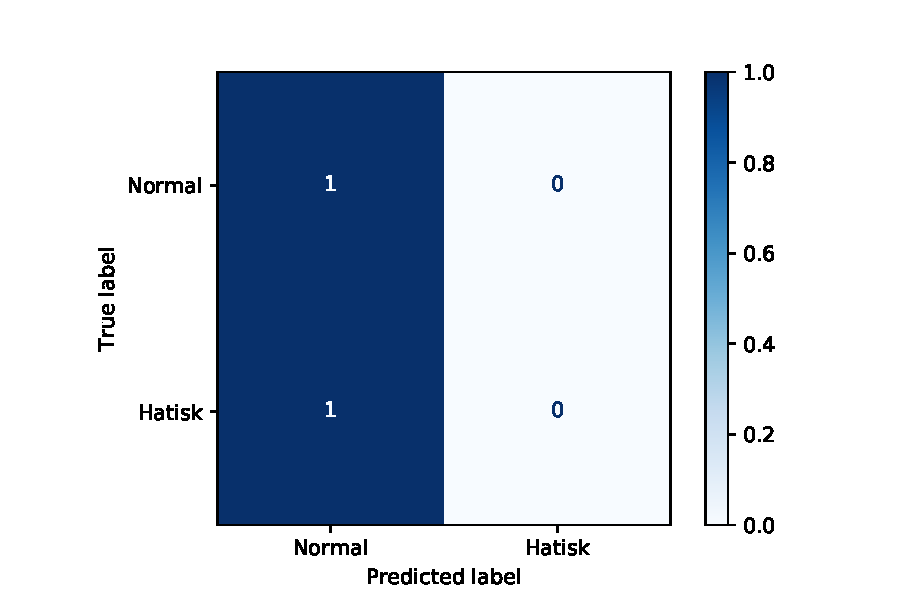
\includegraphics[width=\textwidth*3/4]{bilstmcharsDanish.pdf}
    \caption{Confusion matrix for the Bidirectional LSTM model in Danish.}
    \label{fig:danlstm}
\end{figure}

For the Ifrågasätt data, it is a bit more complex. The logistic regression classifier with TF-IDF features has a worse F1-score than a naïve classifier that only predicts one class. Undersampling also gives no benefit to the TF-IDF model, most likely due to the relative simplicity of the model. Moreover, even if the more complex models do improve the score with undersampling of the majority class, they fail to reach the performance of TF-IDF model on the other datasets. 

To better understand what is happening with the results,  Figures \ref{fig:tfidf},  \ref{fig:undertfidf}, \ref{fig:underBiLSTM}, and \ref{fig:underBERT}  show the confusion matrices for four of the models. The TF-IDF model performs similarly for the two classes with regards to recall, but the more complex models have issues with achieving a high recall for the offensive class. Combined with the strong class imbalance shown in Table \ref{tab:deskriptiv} and the high accuracy in Table \ref{tab:monolingual}, this means that there is a very high precision for the majority class of normal comments but a much lower precision for the minority class of offensive comments. The precision for the BERT model is in fact 99.1\% for the non-offensive comments while only being 8.0\% for the offensive comments.

\begin{figure}[t]
    \centering
    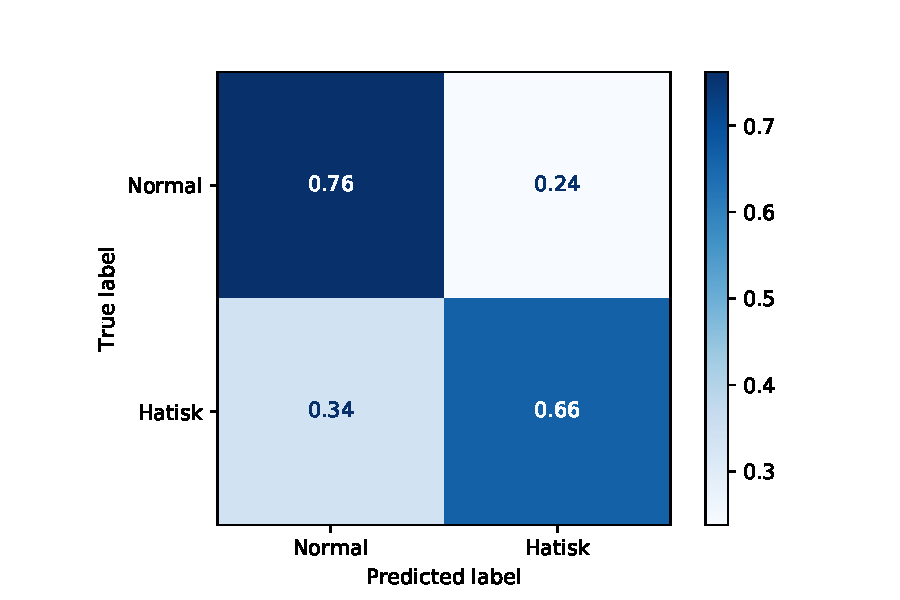
\includegraphics[width=\textwidth*3/4]{tfidf.pdf}
    \caption{Confusion matrix for the logistic regression model in Swedish.}
    \label{fig:tfidf}
\end{figure}

\begin{figure}[t]
    \centering
    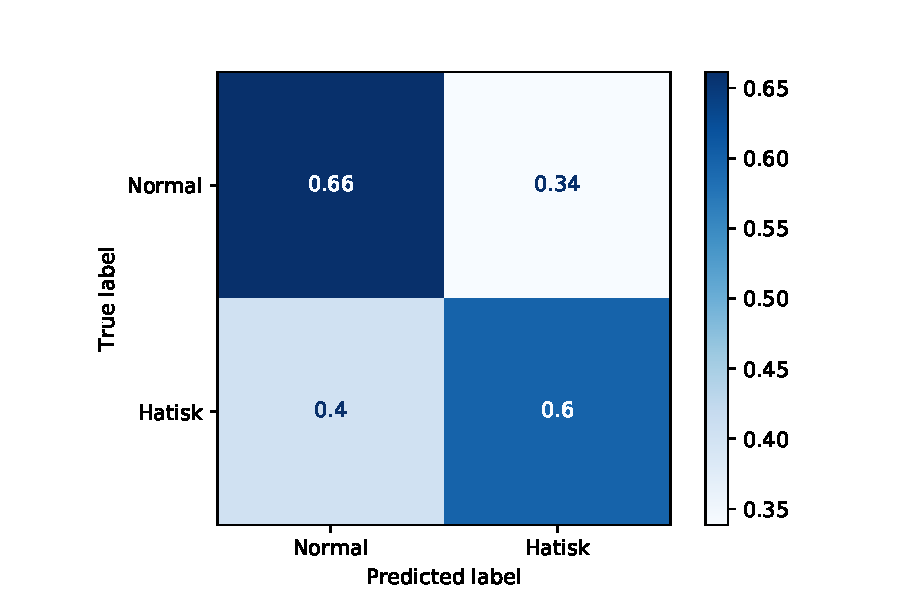
\includegraphics[width=\textwidth*3/4]{undersampledtfidf.pdf}
    \caption{Confusion matrix for the undersampled logistic regression model in Swedish.}
    \label{fig:undertfidf}
\end{figure}

%\begin{figure}[t]
%    \centering
%    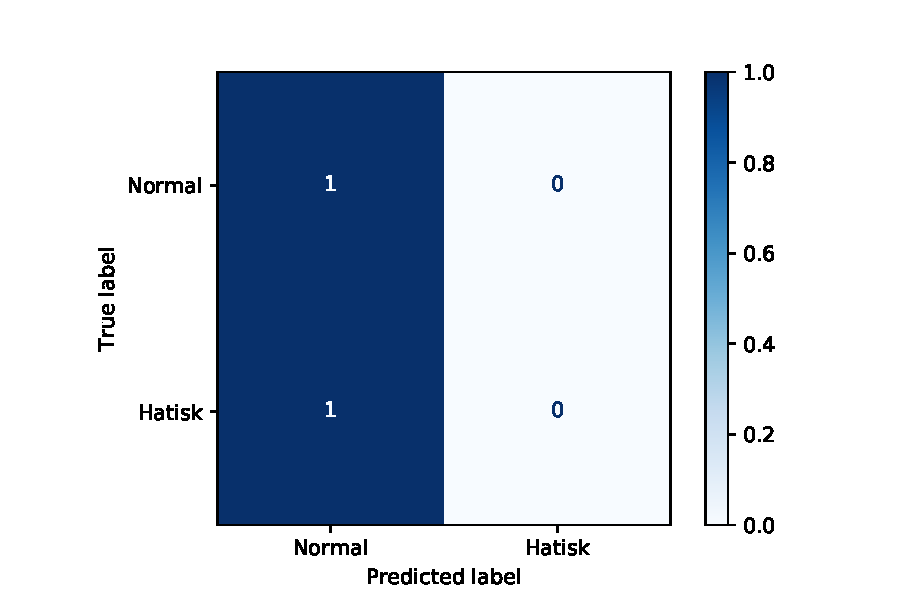
\includegraphics{bilstmIfragasatt.pdf}
%    \caption{Confusion matrix for the bidirectional LSTM model in Swedish.}
%    \label{fig:BiLSTM}
%\end{figure}

\begin{figure}[t]
    \centering
    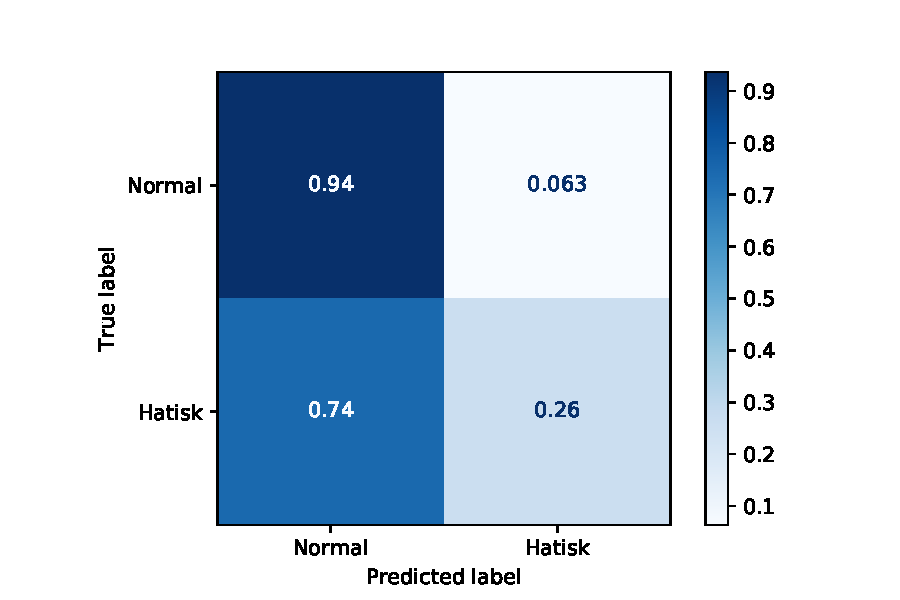
\includegraphics[width=\textwidth*3/4]{bilstmcharIfragasattundersampled.pdf}
    \caption{Confusion matrix for the undersampled bidirectional LSTM model in Swedish.}
    \label{fig:underBiLSTM}
\end{figure}


\begin{figure}[t]
    \centering
    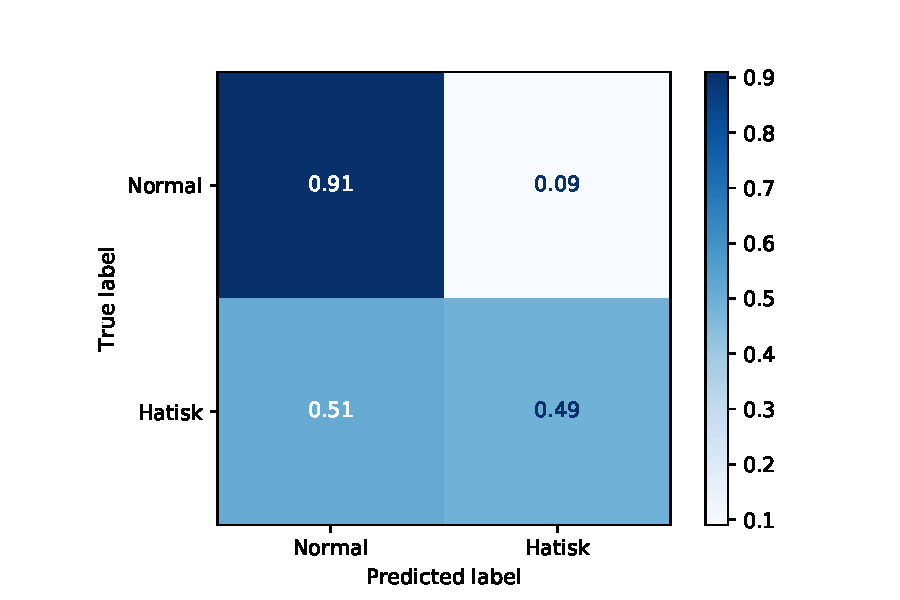
\includegraphics[width=\textwidth*3/4]{bertIfragasattresampled.pdf}
    \caption{Confusion matrix for the undersampled BERT model in Swedish.}
    \label{fig:underBERT}
\end{figure}

%\begin{figure}[t]
 %   \centering
%    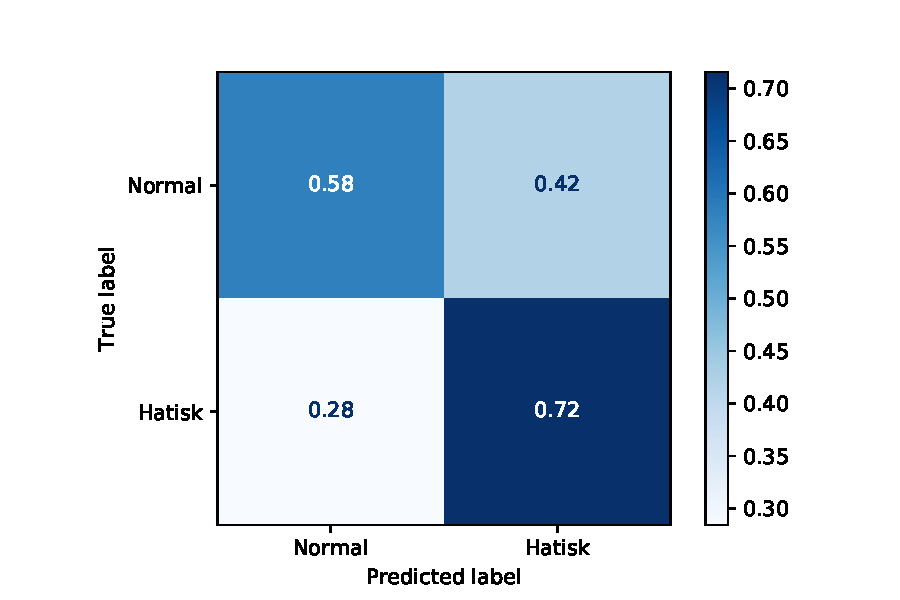
\includegraphics{tfidfOLID.pdf}
%    \caption{Confusion matrix for the logistic regression model in %English on the OLID dataset.}
%    \label{fig:OLIDtfidf}
%\end{figure}
%\begin{figure}[t]
 %   \centering
 %   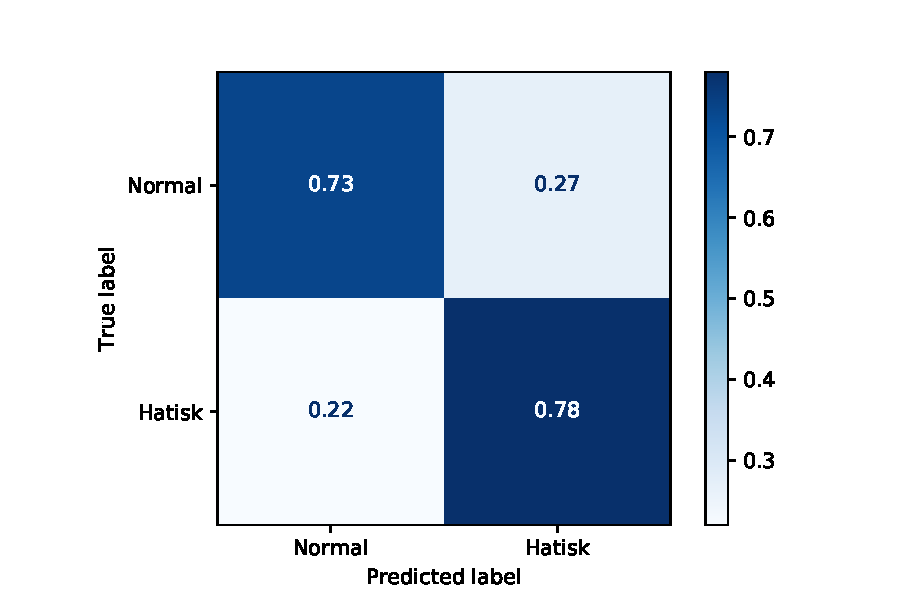
\includegraphics{bilstmOLID.pdf}
 %   \caption{Confusion matrix for the bidirectional LSTM model in %English on the OLID dataset.}
 %   \label{fig:OLIDLSTM}
%\end{figure}

\section{Cross-lingual text classification}

The results for the cross-lingual text classification shown in Table \ref{tab:crosslingual} show that we can train an XML-RoBERTa model even without labeled data in the target language. The results for the Danish dataset with only English training is better than what can be achieved with TF-IDF model trained on the Danish OffensEval dataset. With some complementing of labeled target language data, the results are almost the same as for the monolingual English dataset using a BERT model from Table \ref{tab:monolingual}.

The results for the target language of Swedish do not meet the same expectations. Slightly better results are achieved without using the data from Ifrågasätt than using the data from Ifrågasätt. The target language resources actually harm the model's performance instead of improving it. This is contrary to what would be expected and the opposite of the experiment with Danish as the target language. 

\begin{table}[t]
\centering
\begin{tabular}{@{}llrr@{}}
\toprule
Training language & Evaluation language & Accuracy & Macro F1-score  \\ \midrule
English $\And$ Danish & Danish & 0.78 & 0.78 \\
%Precision of non-offensive: 0.96 Precision of offensive: 0.60
%Recall of non-offensive: 0.94 Recall of offensive: 0.61
English & Danish & 0.63 & 0.64 \\
%Precision of non-offensive: 0.95 Precision of offensive: 0.31
%Recall of non-offensive: 0.74 Recall of offensive: 0.77
English $\And$ Swedish & Swedish & 0.98 & 0.51 \\
%Precision for label 0 is 0.9907589252972383
%Recall for label 0 is 0.8590152120000283
%F1-score for label 0 is 0.9201955753351045
%Precision for label 1 is 0.05565546616185518
%Recall for label 1 is 0.509090909090909
%F1-score for label 1 is 0.10034129692832766
%Macro average F1-score is: 0.5102684361317161
English & Swedish & 0.97 & 0.52 \\
%Precision for label 0 is 0.98537467775955
%Recall for label 0 is 0.9508487512543993
%F1-score for label 0 is 0.9678038885652015
%Precision for label 1 is 0.04712974380052062
%Recall for label 1 is 0.1469457496796241
%F1-score for label 1 is 0.07136929460580912
%Macro average F1-score is: 0.5195865915855054
\bottomrule
\end{tabular}
\caption{Results for the crosslingual models.}
\label{tab:crosslingual}
\end{table}


%\begin{figure}[t]
%    \centering
%    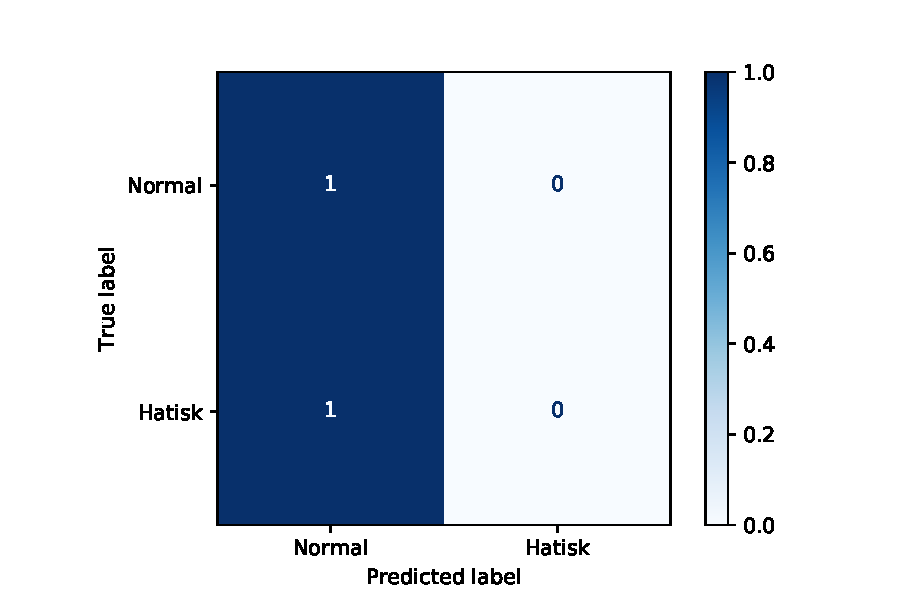
\includegraphics{bilstmIfragasatt.pdf}
%    \caption{Confusion matrix for the bidirectional LSTM model in Swedish.}
%    \label{fig:BiLSTM}
%\end{figure}

\chapter{Discussion and Conclusion}


\section{The Ifrågasätt dataset}

The performance on the Ifrågasätt data is lackluster and would be considered bad for most datasets. Even if one assumes that the task of classifying the comments at Ifrågasätt are harder than the offensive tweets of the OffensEval data, the 0.37 F1-score difference is too large to be explained solely by this. The unexpected result on the cross-lingual experiment with the Ifrågasätt data and the English OffensEval data shows that having more of the Ifrågasätt comments in the training data doesn't necessarily help the performance of the model. 


More data should, with diminishing returns, almost always be useful for a machine learning model. This should be even more true when the training data that is added in the same language as the evaluation data and thus more applicable to the evaluation data than the English language data. This decrease in performance when adding the Swedish data points to some underlying issue with either the implementation or the dataset. Given that the model works as expected for the English and Danish datasets, the problem is likely to be found in the dataset. This is somewhat expected from the analysis of the inter-annotator agreement found in the dataset chapter. There are a lot of comments on the platform, but the consistency between the annotations isn't high enough for the data to be utilized to its full potential. 

This doesn't mean that the classifiers are useless. The better performing bidirectional LSTM and BERT models can still be considered useful. There is a high precision for the non-offensive comments, but the large difference in F1-score and accuracy means that the model has failed to learn how to effectively discriminate between the classes.  Even if the models do not discriminate effectively, they do well at finding most of the non-offensive comments. Therefore it is a working tool for sorting out and prioritizing a subset of the comments that are hateful. 

Since the comments on Ifrågasätt, and presumably most other newspapers are eventually all read and confirmed to fit on the platform, these models provides an automatic way of finding some of the hateful comments quicker than labeling them in a random order would do. For example, by prioritizing the comments classified as hateful by the BERT model one can find 50\% of the hateful comments by reading less than 10\% of the comments that are published. It is clear that the low precision is still a problem because one would need to read an average of 15 comments for every hateful comment to be found, but this is still useful to remove some comments earlier. To accomplish more it is likely that the issues with the dataset need to be addressed.

The quality of the dataset mostly falls outside the scope of this thesis, but if the moderators' daily work should be better suited for the use in classifiers in the future, this should be addressed. There are several possible paths to make the inter-annotator agreement higher. More stringent moderator training would make it more likely they understand the guidelines similarly. This can be implemented for example as a training dataset that a moderator has to annotate correctly enough to begin working. Some sort of ``supervision'' between the moderators can be added where they, knowingly or unknowingly, label data points that someone else has labeled before to look at performance in real time to make sure that their interpretations do not shift too greatly in time. The moderators could put the comments into strict categories instead of relying on the free text moderating reason for comments, which would also remove any errors introduced by the categorization method. 

It should also be clear that the annotation task being harder is not really an assumption but also a reasonable deduction from the moderators noting that the task is harder without context. The moderators, when annotating comments, take things such as the context of the comment, how language evolves over time and what newspaper it is written on, This is information the model has no concept. The models as implemented have no information about the metadata of the comment (what newspaper it is written on) or what the comment is responding to, which the annotators does. This means that even taking into account the lower inter-annotator agreement on the dataset, classifiers that do not model these things should perform worse than on other toxicity datasets with equivalent inter-annotator agreement. 

A model could possibly take these things into consideration and I carried out some experiments to analyze this point. In an effort to model stricter moderating criteria for certain newspapers, I tried to incorporate newspapers embeddings into the bidirectional LSTM model, but I found no difference in result from the one reported in Table \ref{tab:monolingual}. In practice, the large number of newspapers means there aren't many comments from the offensive category that are in the training set. When this is combined with the heavy undersampling that was required to make the models converge, the lack of benefit is reasonably explained. Not only does the quality of the annotated comments prevent good performance, but the large class imbalance comes in again as a factor in making the classification task harder. The class imbalance makes it hard for a deep learning model to learn from the entirety of the dataset.  

It could also be possible to take into account earlier comments in the comment chain, the text and headline of the newspaper article itself as some sort of features, but this was left for future work.

\section{Cross-lingual text classification}

The results for the English-Danish cross-lingual text classification show that cross-lingual text classification is a surprisingly mature field. Offensive text classification requires a high level of understanding of language and even for humans, it hard to consistently categorize texts as found in the dataset chapter. 

That a model can not only understand these categories somewhat well, but also does it cross-lingually without target language data bodes well for implementing models for dataless languages. As can be seen in the results for the monolingual Danish models in Table \ref{tab:monolingual}, the deep learning models fail to give meaningful results with only a modest amount of data. That the cross-lingual model overcomes this problem is good news. This means that, if one has a starting point of having a good dataset of offensive text in one language, this data can be of use in other languages. 

This opens up a quite simple procedure for expanding the XLM-RoBERTa model into other languages. For good results in new languages, annotators that can understand the new language are necessary, but they do not need to pre-annotate a large corpus. Even without data in the language, the model will produce useful results. The annotators can start with this model and recategorize those comments that the model classified incorrectly. They will over time create a dataset that can be used to retrain the model. Table \ref{tab:crosslingual} shows that the performance of the model will quickly ramp up without annotating a lot of comments and approach the values of a monolingual BERT model. A small starting set of data  made the results similar to the results of the BERT model in the English language. 

This however assumes that the annotated data has a high inter-annotator agreement. As shown from the cross-lingual experiment with the Ifrågasätt data, more data isn't always better if it is of worse quality than the earlier data. I once again stress the importance of moderators internalizing the guidelines similarly for a classifier to have a high performance.

Some caveats should be placed in that the experiment isn't necessarily applicable to all language pairs. Many other pairings might have worse results. In the XLM-RoBERTa model, the training text sizes for different languages are not evenly distributed and English is the language with the most training data \citep{DBLP:journals/corr/abs-1901-07291}. As English is a high-resource language in this context, reasonably it should have one of the better cross-lingual capabilities as well. 

Even if Danish has a lower amount of training data than English, it has more data than some other languages in the training set and is linguistically quite close to English. Both are Germanic languages with similar grammar and while the vocabularies are different, they are sometimes very similar. All else being equal, it should be easier to model semantic similarities in languages with recent common ancestors than those without. The results would likely have not been as good for example if the Arabic OffensEval dataset was used to complement the Danish data. 

For this reason, it would also have been interesting to try to complement the Danish OffensEval data with the Ifrågasätt data in Swedish. While these languages are very close linguistically, they together make up a relatively small portion of the data that was used in training for the XML-RoBERTa model. An experiment testing this would be more applicable for future use in Ifrågasätt Media Sverige AB, but also tell us more about how much pre-training data is required to achieve good cross-lingual capabilities. This is left as future research.






% Should use consistent formatting when it comes to Names ("FirstName LastName", or "F. LastName")
%\printbibliography
\makebibliography{referenser}

\end{document}
